\chapter{プロトタイピング}
\label{prototyping}
本研究では、「手指の変換表現」についての\ref{prototyping_concept_making}節のような動機を起点に「人馬一体感」のデザインが目的となり、修士作品《Grasp(er)》を制作した。ここでは、その過程にあるプロトタイピングについて説明する。
本章ではまず、それらのプロトタイプについて、「形状」、「マッピング」、「時間操作」、「ボール操作」の観点から分類する。その上で、これらのプロトタイピングFelsの分類を用いて分析し、「人馬一体感」を具現化する表現となりうるものについて述べる。

\section{制作環境と記録方法}
「手指の変換表現」におけるプロトタイプを評価する上では、次のような事項について配慮する必要がある。まず、単に動きを記録・観察するのみならず、インタラクションにおける主観的な経験が重要であるため、何度も体験できる状況を確保することである。さらに、実装を通して仕組みを理解している制作者にとっては、\ref{prototyping_concept_making}節で示したような、探索的に動かすことの中でその仕組みを解釈していくような経験をすることができないため、制作者ではない人の意見が重要になる。

こうした要求を踏まえて、プロトタイプはWebブラウザ上で動作し、カメラ映像のみでハンドトラッキングを行うといった、ソフトウェアの点でもハードウェアの点でも簡易に動作環境を再現できる制作環境を構築した。インターフェースには、Vercel社が提供するWebアプリケーションフレームワークであるNext.jsを使用し、ハンドトラッキングにはTensorflowの開発グループがサンプルとして提供するhand-pose-detection\footnote{\url{https://github.com/tensorflow/tfjs-models/tree/master/hand-pose-detection}}を用いた。

\begin{figure}[H]
  \centering
  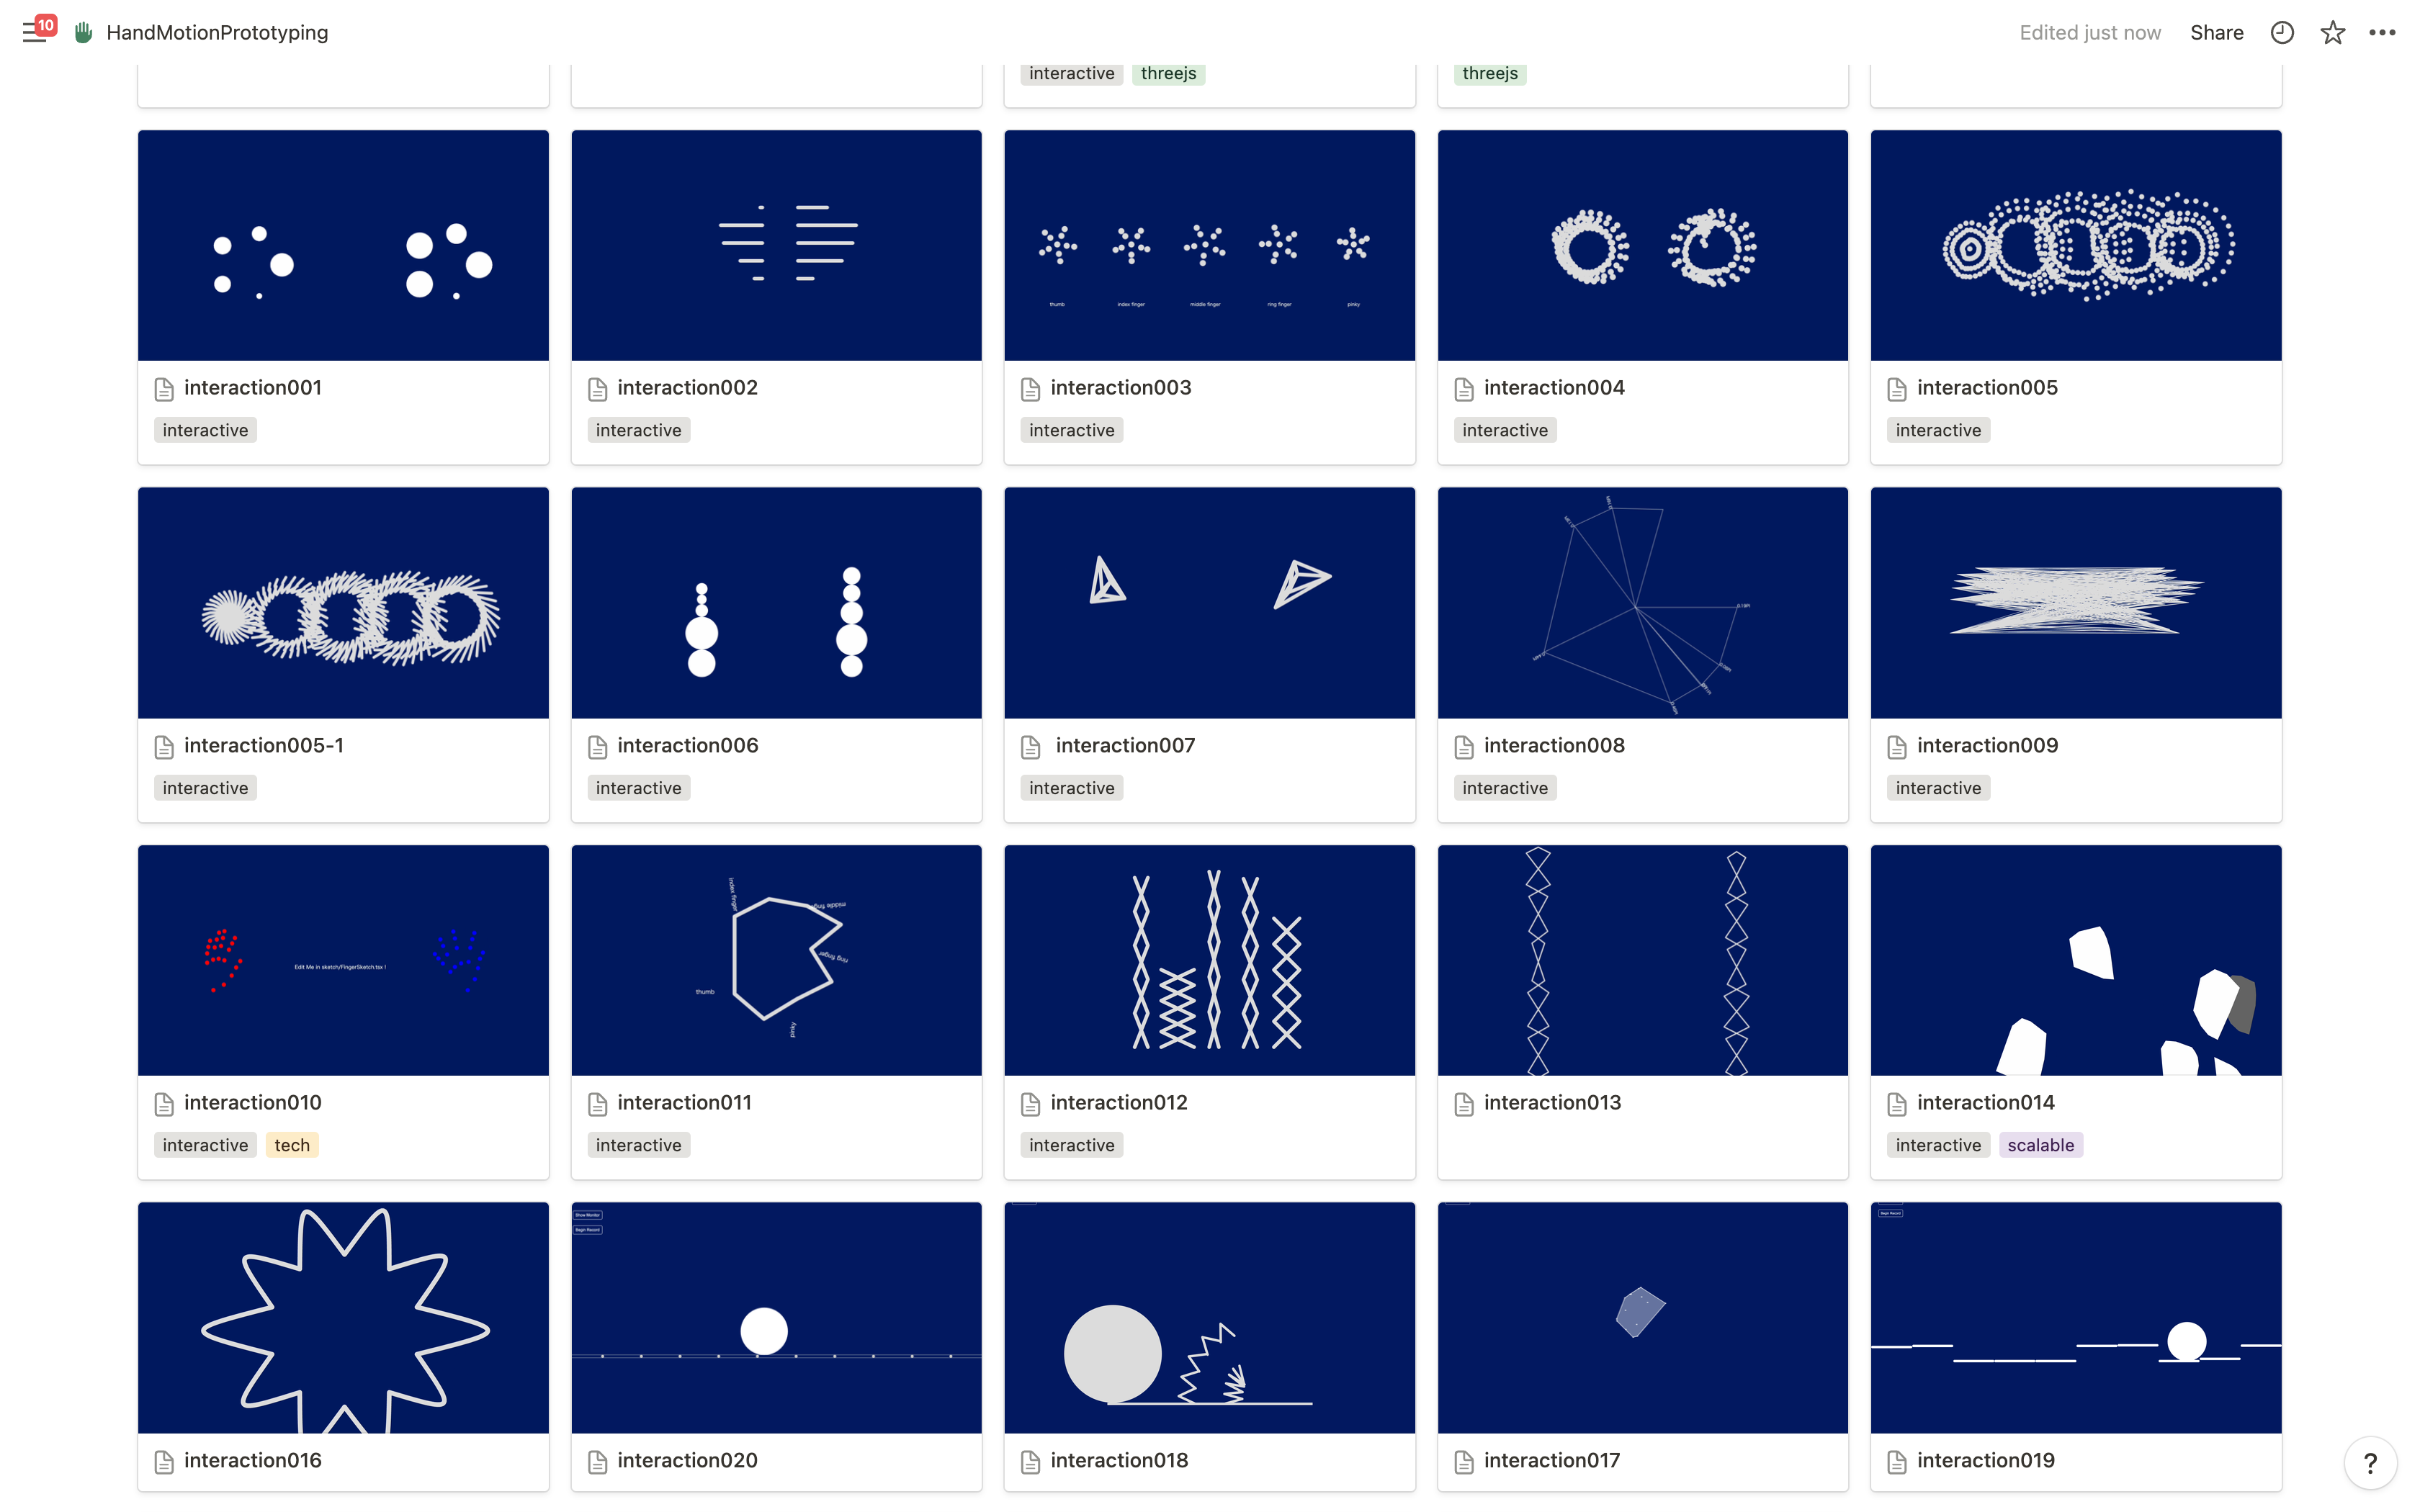
\includegraphics[width=15cm]{img/prototype_overview.png}
  \caption{プロトタイプのインデックスページ}
  \label{fig:prototype_overview}
\end{figure}

\section{プロトタイプの分類}
修士作品の制作に至るまでに、2022年6月から2023年10月までの期間で、表現の可能性や応用を探る目的で総計60パターンのバリエーション、並びに計6回のプロトタイプの展示を実施した。ハンドトラッキングによって推定された姿勢情報は、下図\ref{fig:keypoints}に示す21個のキーポイントで表現される。こうしたキーポイントの情報をもとに、その配置や関係性といった構造、そしてそれをどのように表現するのか、といった点から変換表現について検討した。先入観で判断しないよう、この段階では先の研究目的を意識せず、このような探索空間の中で思いつく限り実装することを重視してプロトタイピングをおこなった。

プロトタイピングは、形状、マッピング、時間操作、ボール操作などの観点から分類することができる。単に形を考えるだけでなく、どのようにマッピングさせるか、そしてどの時間の動きを用いるか等、さまざまな変換方法を検討した。本章ではこれらの分類に基づいて、制作したプロトタイプについて概観する。

\begin{figure}[H]
  \centering
  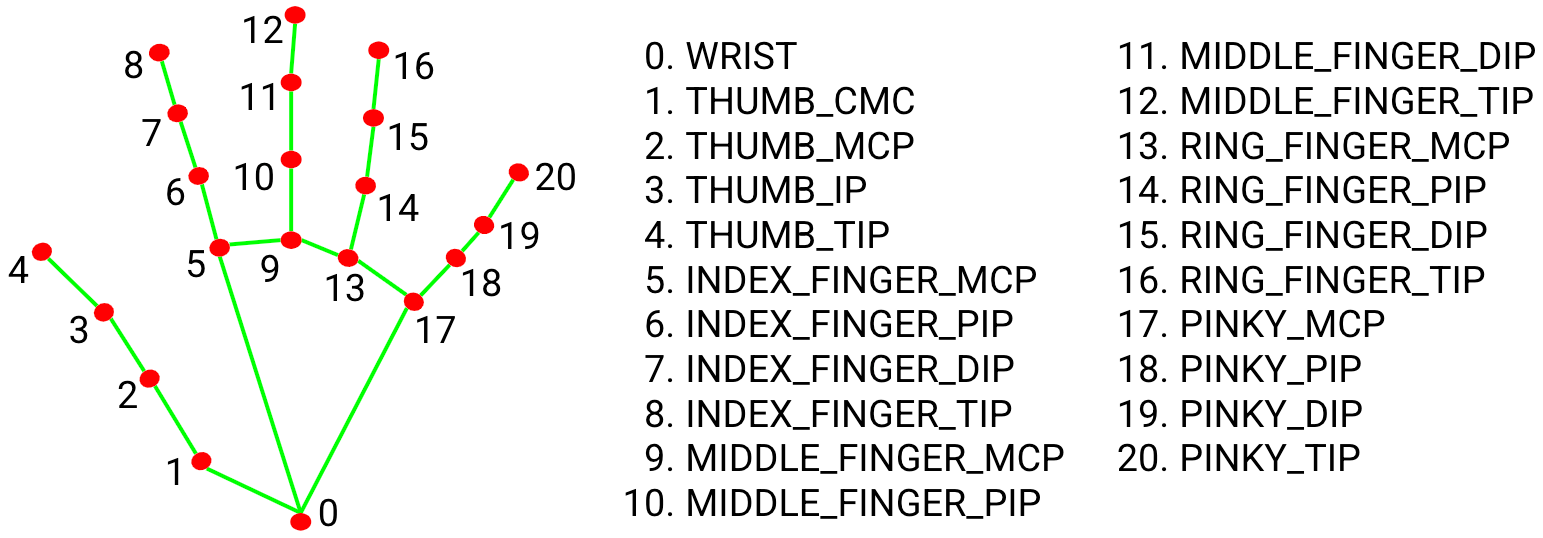
\includegraphics[width=15cm]{img/hand_keypoints.png}
  \caption{モデルを用いて表現されるキーポイント:hand-pose-detectionモデルのリポジトリより引用}
  \label{fig:keypoints}
\end{figure}

\subsection{形状}
形状については、指を1つのユニットとして捉えて、ユニット自体の形状やそれらをどのように関連づけるのかについて検討したもの、そうした枠組みとは無関係に制作したものとの2つに分類して説明する。
\subsection*{指をユニットと捉えたバリエーション}
キーポイントの情報を指ごとに分割して捉え、指一本の中で生じる動きを一つのユニットと捉えてバリエーションを展開した。以下の図\ref{fig:unit_valiation}に示す「ドット」や「ライン」は指のキーポイントを点群として離して出力するか、一つの線として繋げて表示するかの違いである。また、「円」、「くの字」、「クロス」などのバリエーションは、指先の\(y\)座標と指の付け根の\(y\)座標の差を評価して、ユニットの高さ(あるいは直径)が変化する。

\begin{figure}[htbp]
  \begin{minipage}[b]{0.5\linewidth}
    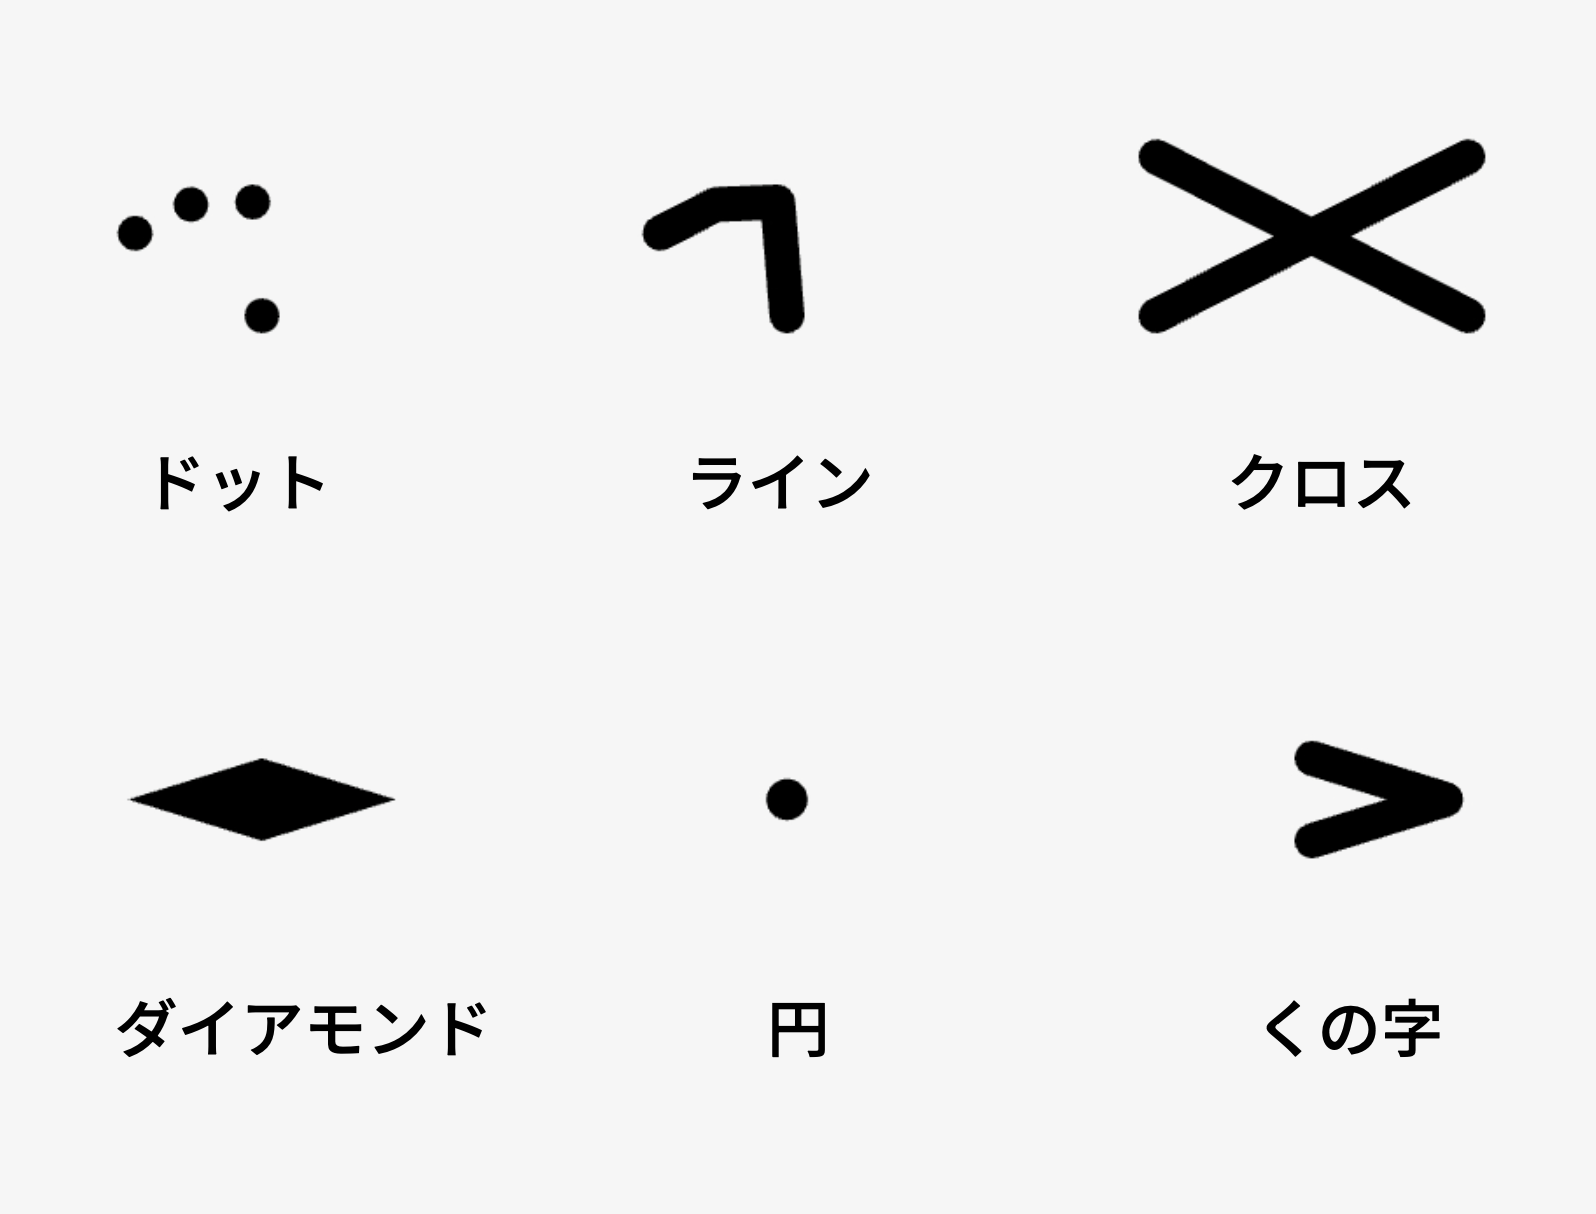
\includegraphics[width=5cm]{img/unit_valiation.png}
    \caption{ユニットのバリエーション}
    \label{fig:unit_valiation}
  \end{minipage}
  \begin{minipage}[b]{0.5\linewidth}
    \centering
    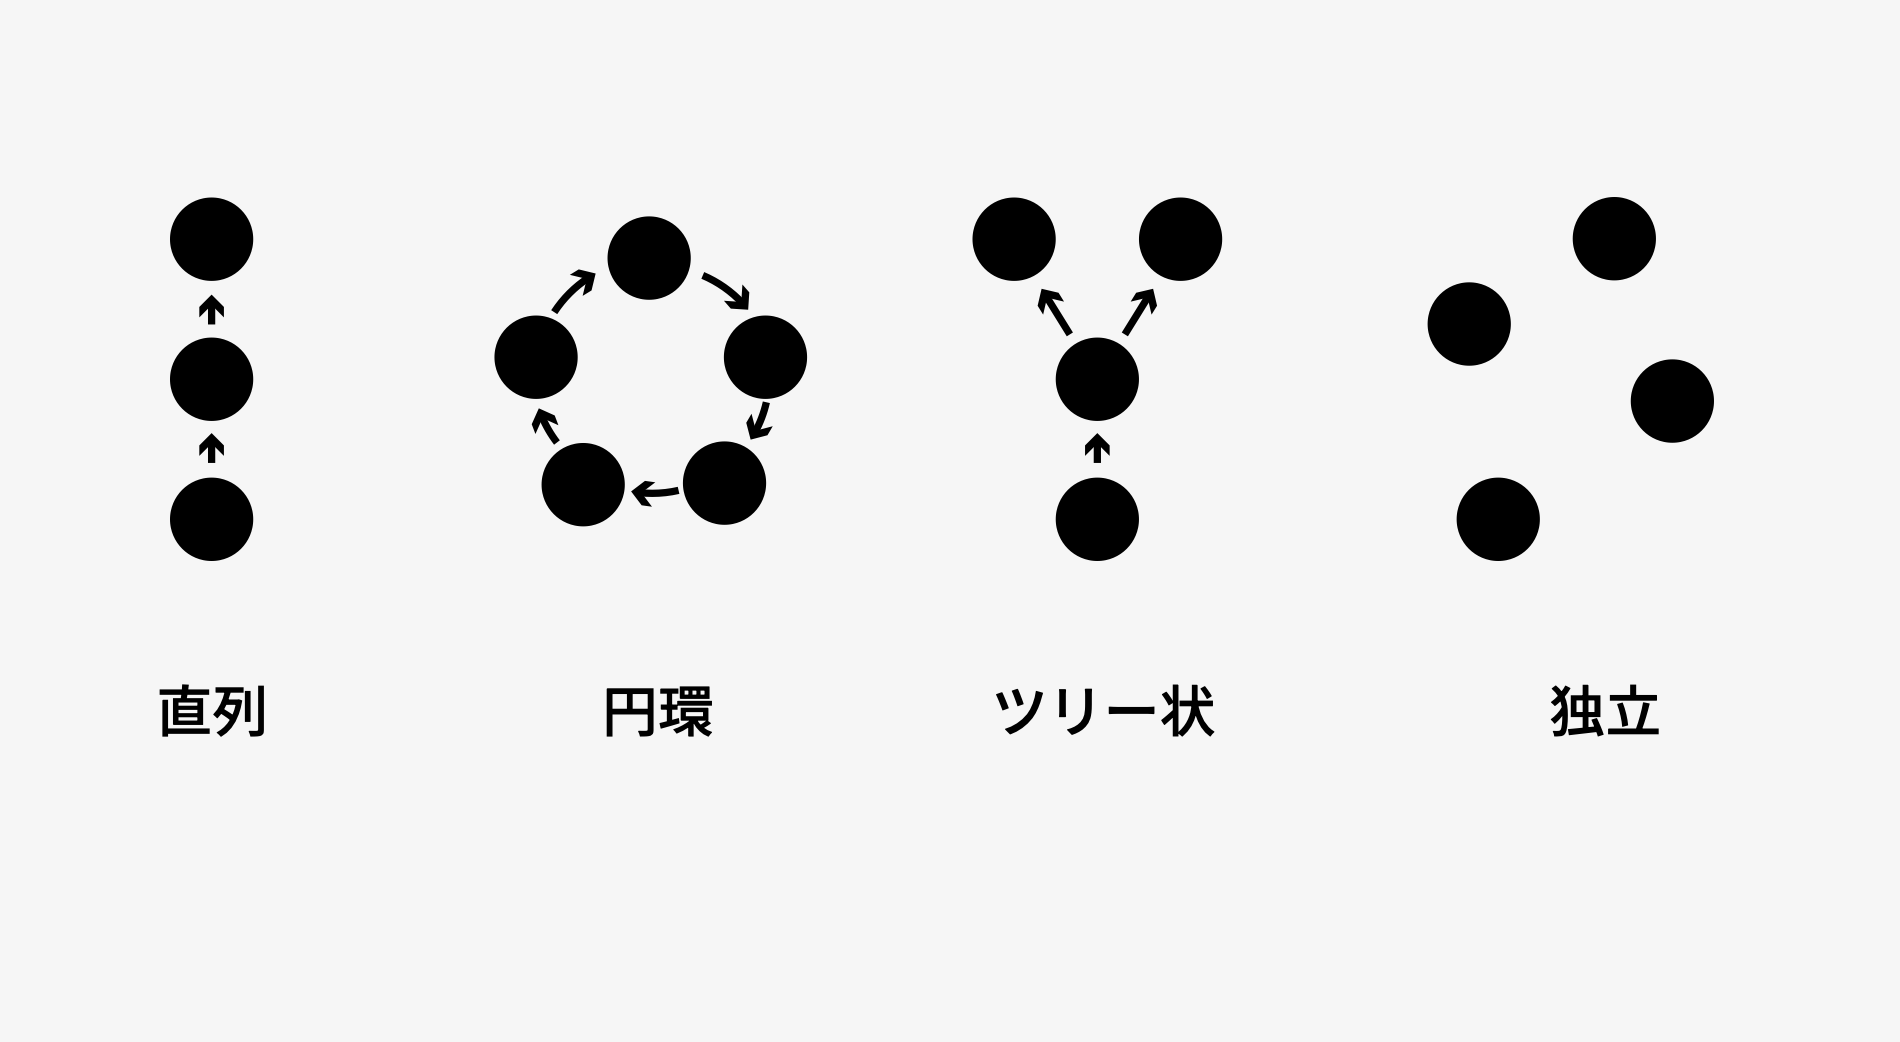
\includegraphics[width=7cm]{img/network.png}
    \caption{繋ぎ方のバリエーション}
    \label{fig:connection_valiation}
  \end{minipage}
\end{figure}

また、これらユニットをいかに繋ぎ合わせて1つの形にするかについても探索を行なった(\ref{fig:connection_valiation})。以下は、同じ「くの字」のユニットについて、「並列に並べたもの」、「片手ずつ直列に繋ぎ、左右の同じ指の高さを結ぶ直線の傾きで回転をかけたもの(B)」、「円形に繋げたもの(C)」の3つのバリエーションである。(図\ref{fig:kunoji_a}, \ref{fig:kunoji_b}, \ref{fig:kunoji_c})

\begin{figure}[htbp]
  \begin{minipage}[b]{0.33\linewidth}
    \centering
    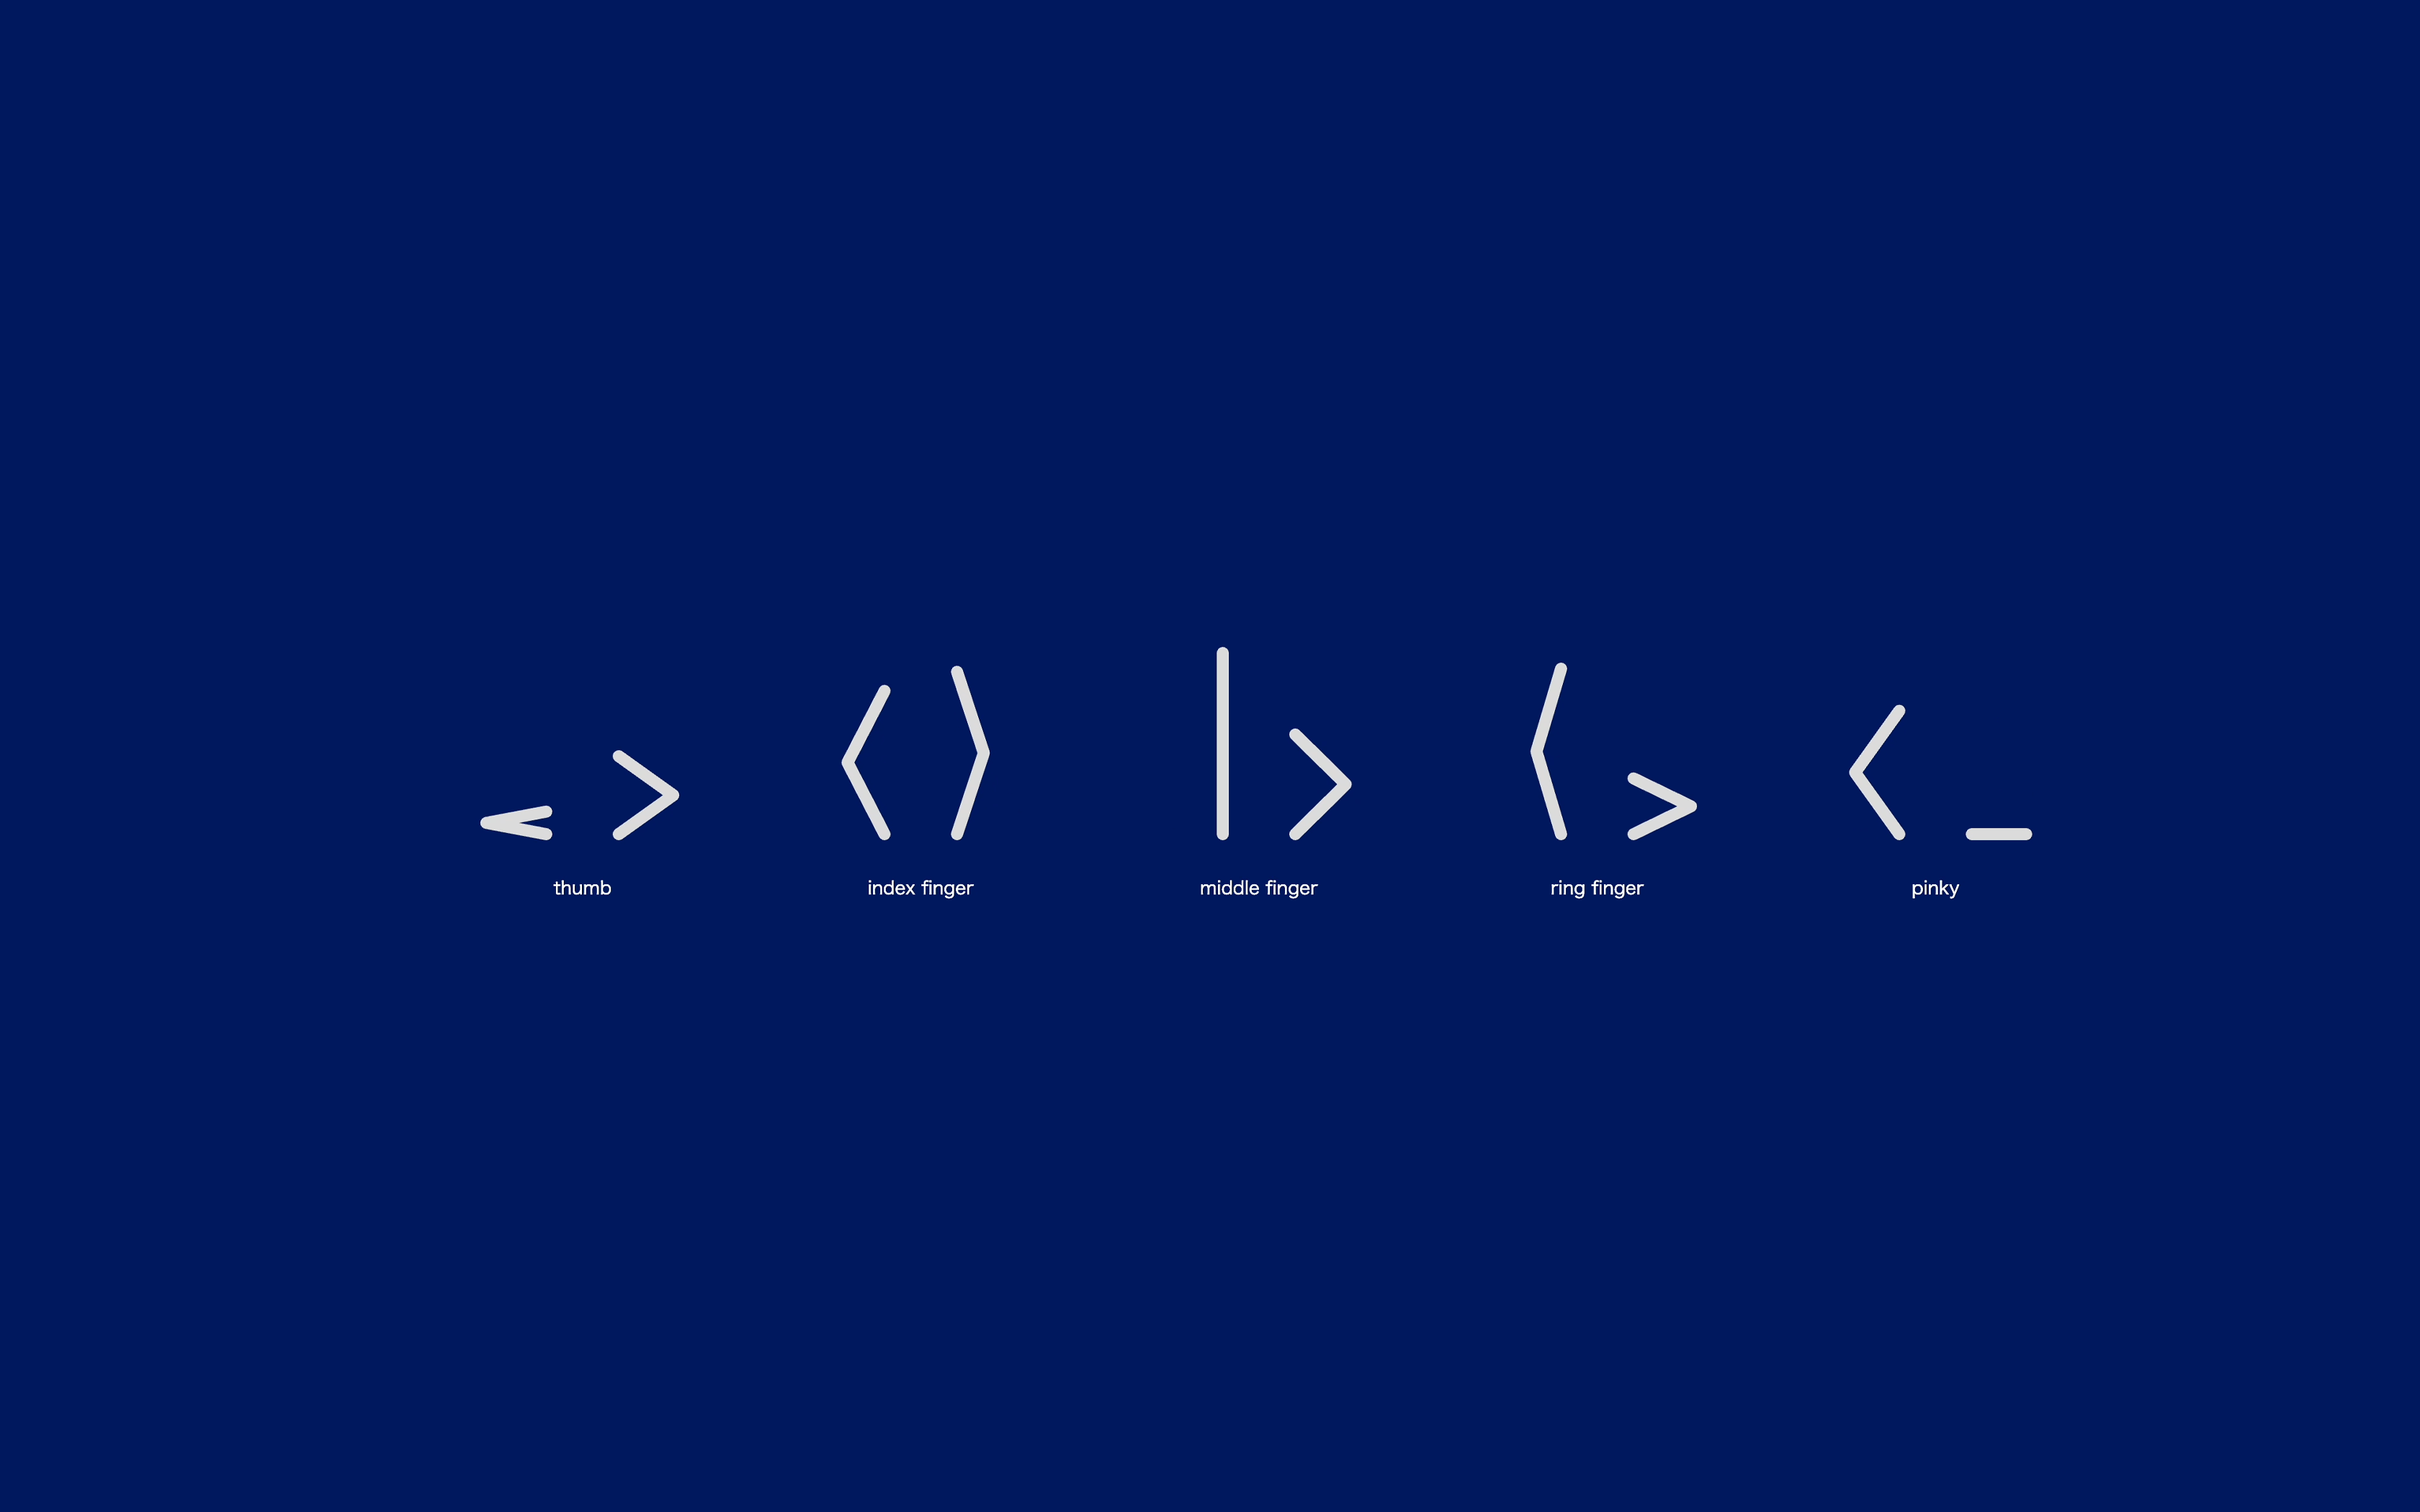
\includegraphics[keepaspectratio, width=4.5cm]{img/kunoji-pararell.png}
    \caption{(A)}
    \label{fig:kunoji_a}
  \end{minipage}
  \begin{minipage}[b]{0.33\linewidth}
    \centering
    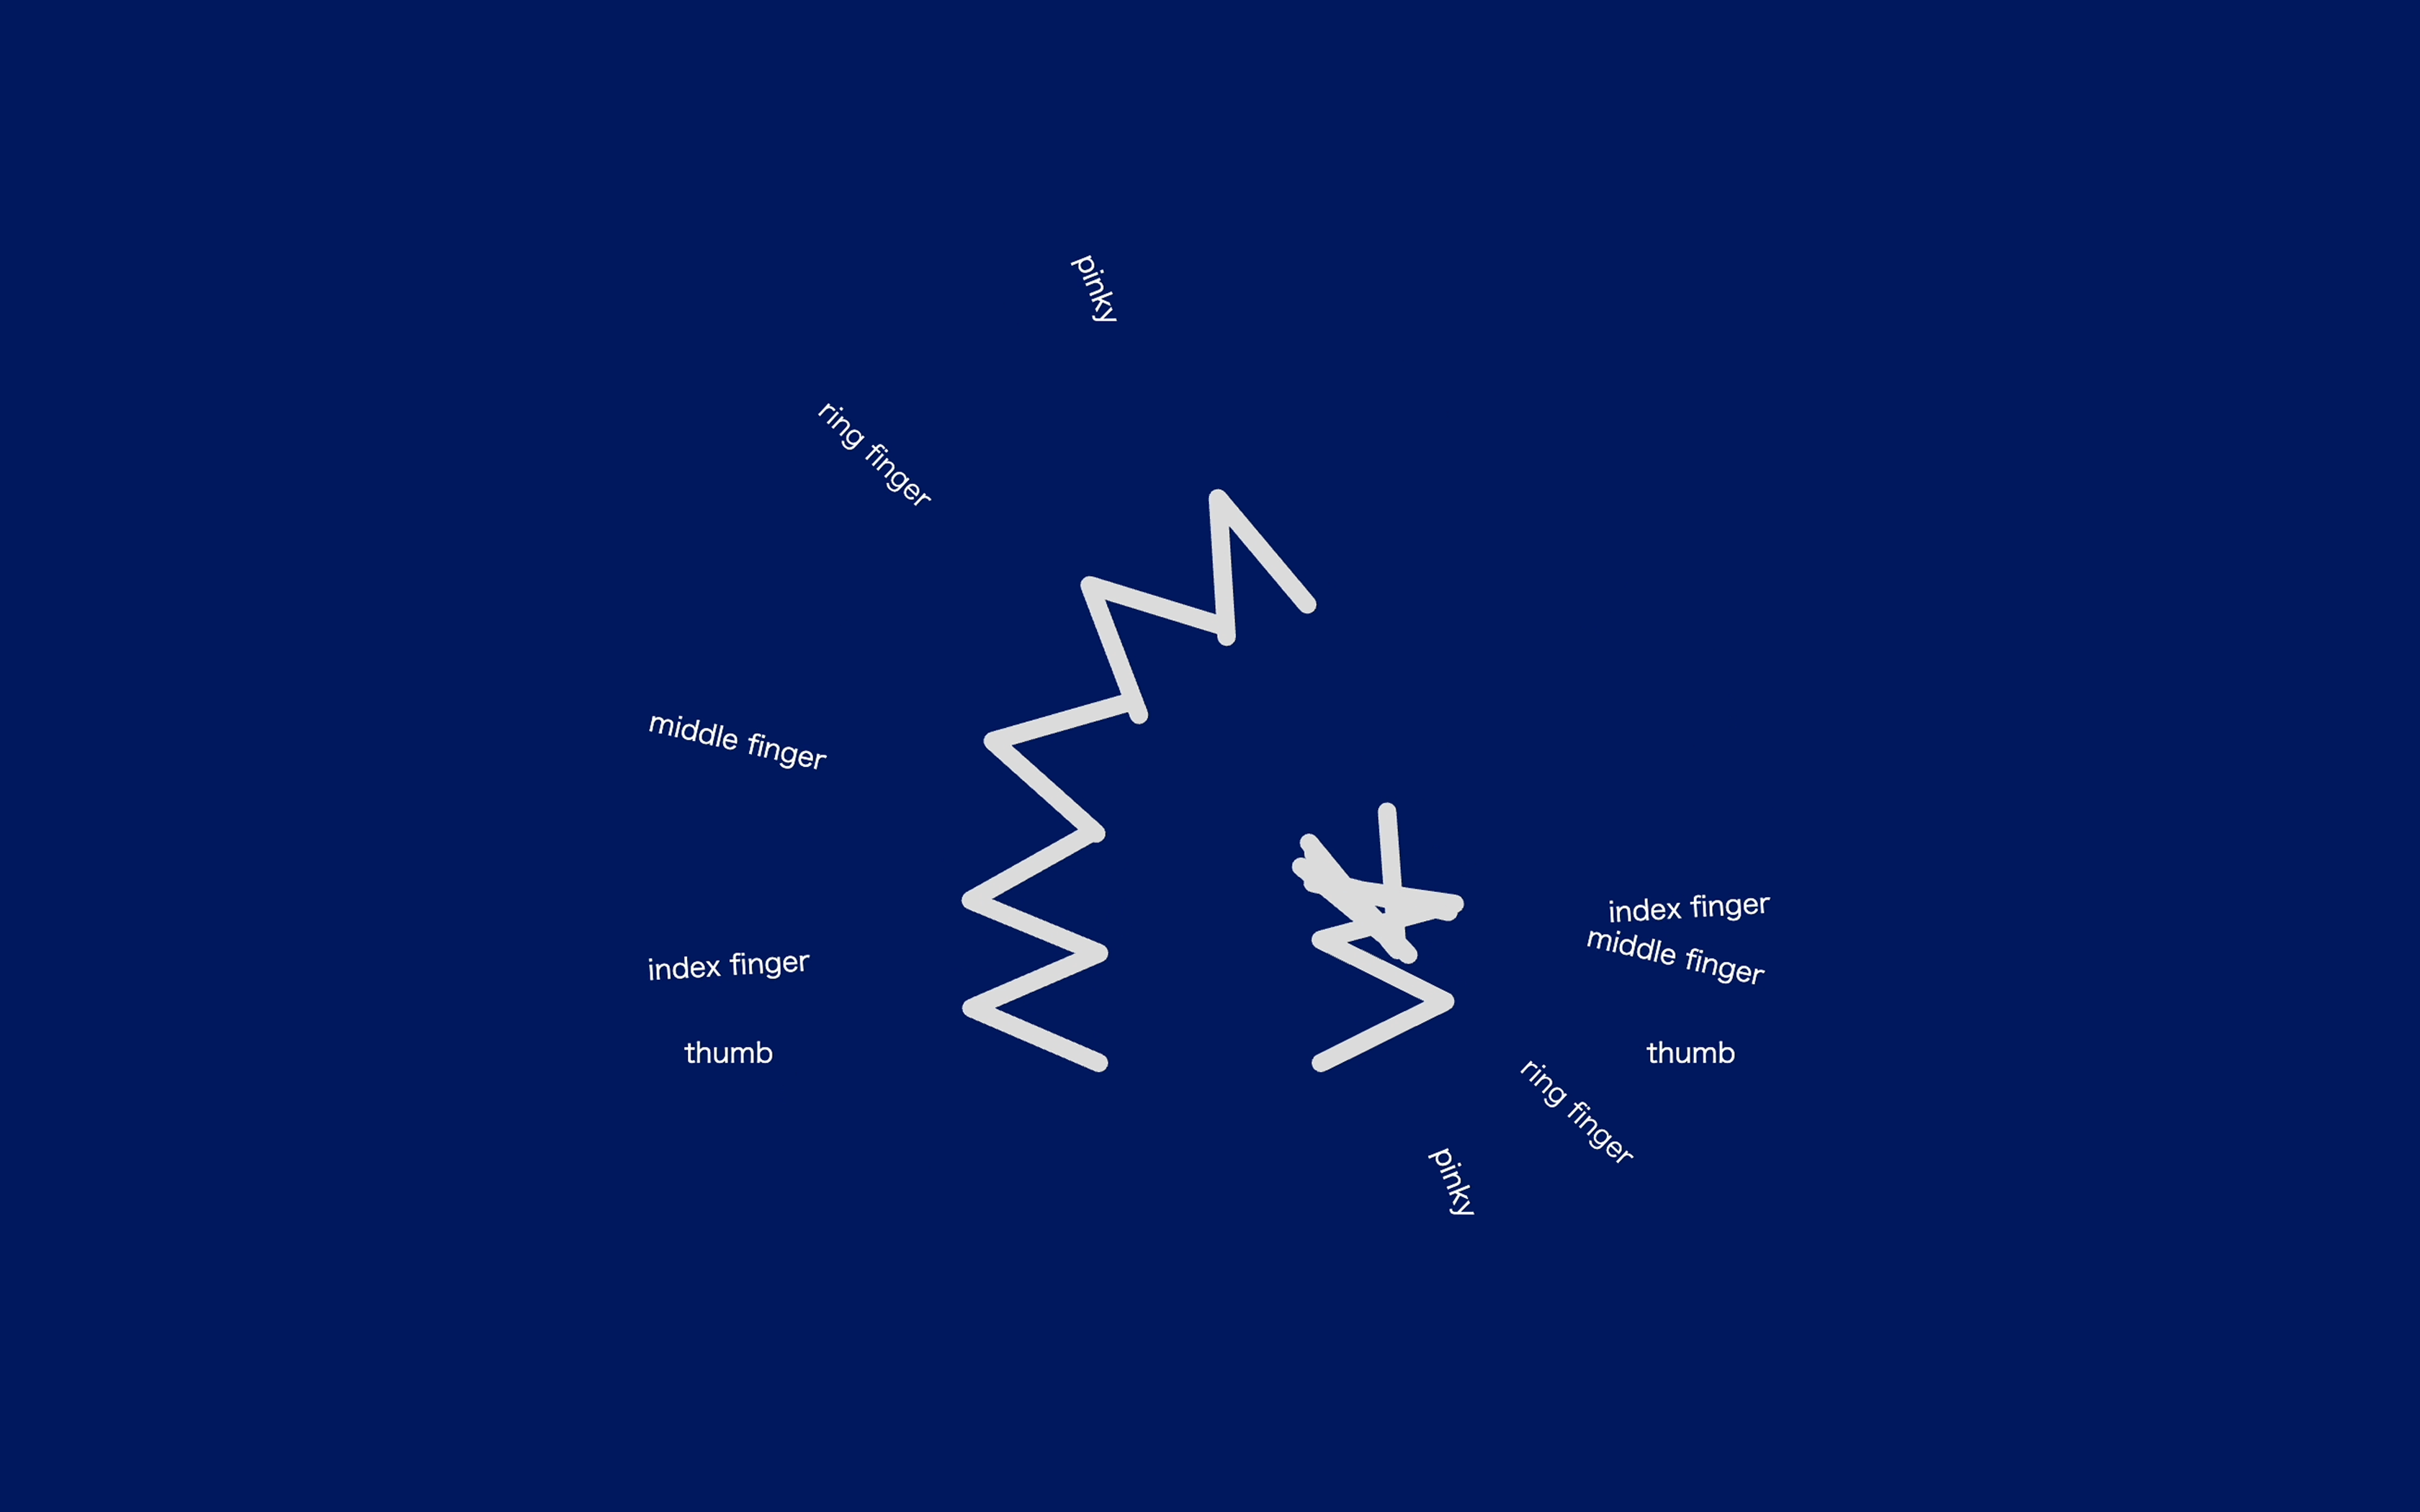
\includegraphics[keepaspectratio, width=4.5cm]{img/kunoji-direct.png}
    \caption{(B)}
    \label{fig:kunoji_b}
  \end{minipage}
  \begin{minipage}[b]{0.33\linewidth}
    \centering
    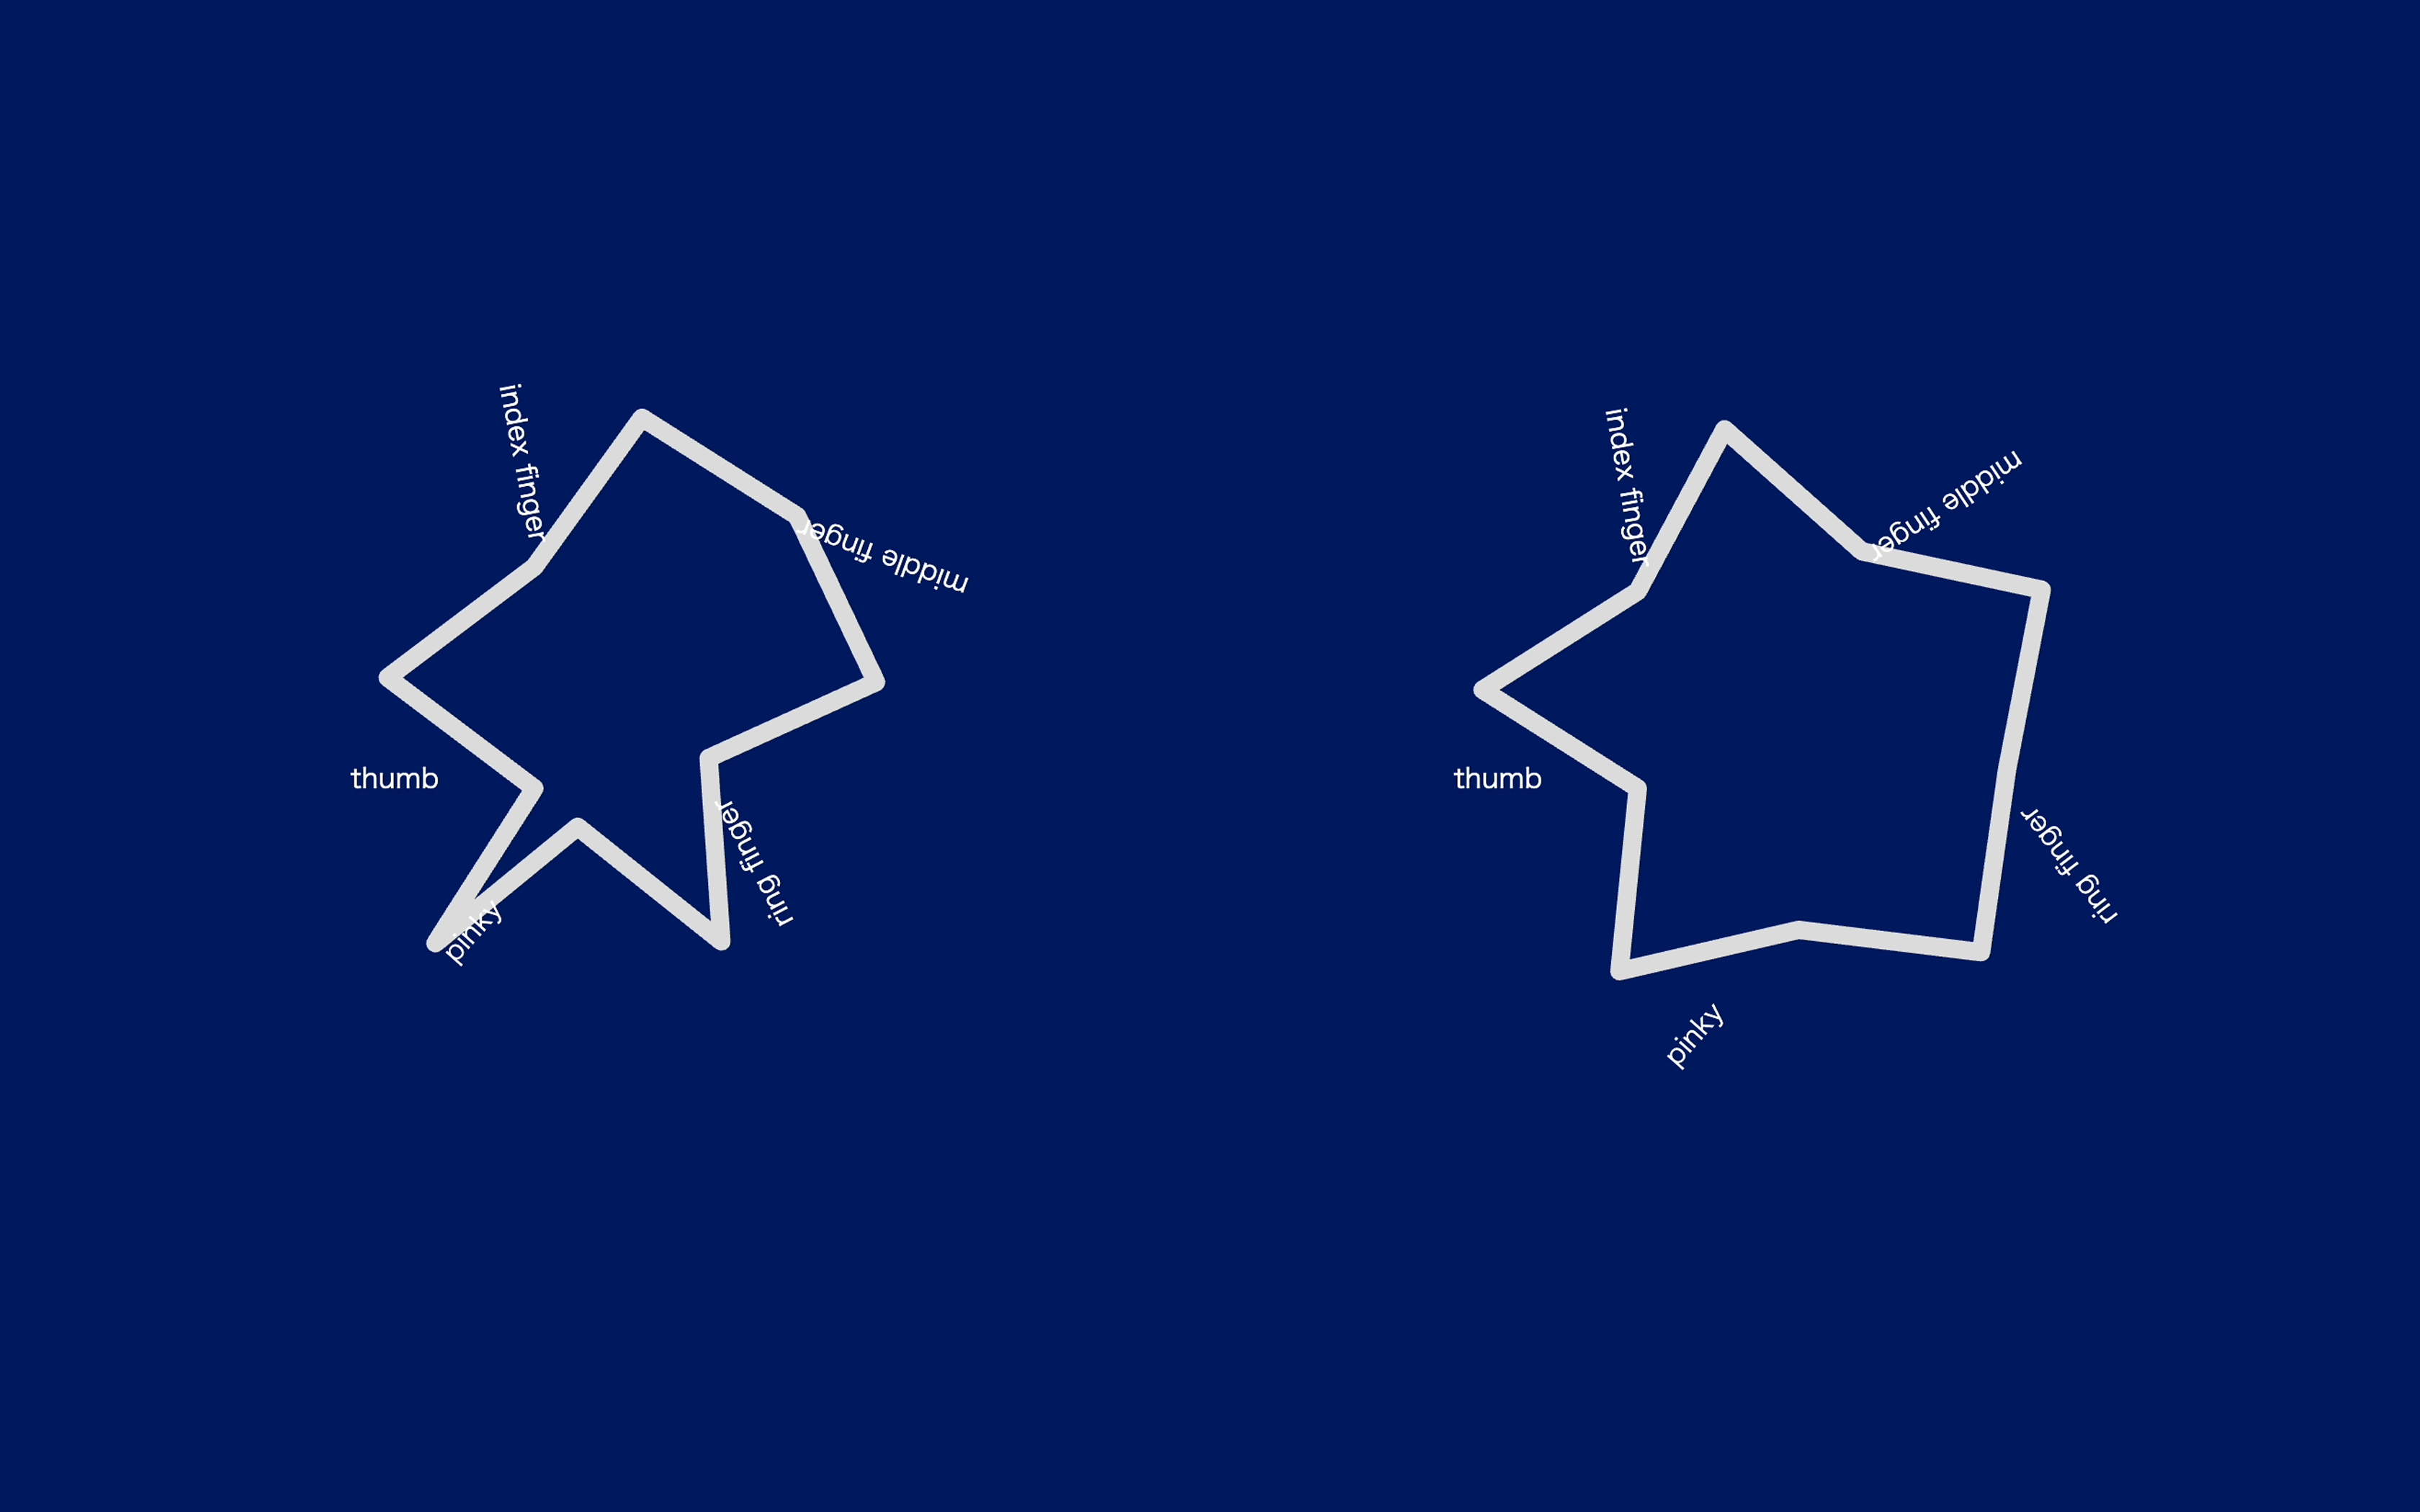
\includegraphics[keepaspectratio, width=4.5cm]{img/kunoji-circle.png}
    \caption{(C)}
    \label{fig:kunoji_c}
  \end{minipage}
\end{figure}

\subsection*{指をユニットとしないバリエーション}
手指の動きを全て包み込む皮膜を「凸包(convex envelope)」のアルゴリズムを用いて実装したり、また指先と付け根の動きだけでなく、指の関節の開き具合を変数として、二等辺三角形の頂角の大きさが変化するバリエーションなどを作成した。

\subsection{マッピング}
マッピングについては、1つの動きが1箇所に対応しているものだけでなく、1つの動きを複数のパーツの動きへと複製したバリエーションなどを作成した。図\ref{fig:networked_finger}に示すプロトタイプ\footnote{\url{https://eee-handpose-playground.vercel.app/work/createNetworkedFingers}}では、指先をクリックすると5本ある指のうちのいずれかの動きを追従する指が、指先に追加されるものである。どの指が付け加わるかはランダムである。そのため指が新しく追加されるたびに、一本一本指を動かして、どこがその指に対応しているのかについて同定する必要がある。

またそのほかに、図\ref{fig:fractal_finger}に示すプロトタイプ\footnote{\url{https://eee-handpose-playground.vercel.app/work/fractalFingers}}は、フラクタル構造で指の動きを配置したバリエーションである。親指の先に人差し指の動きが複数分岐し、さらに人差し指の先から中指の動きが複数分岐して配置される。

\begin{figure}[htbp]
  \begin{minipage}[b]{0.5\linewidth}
    \centering
    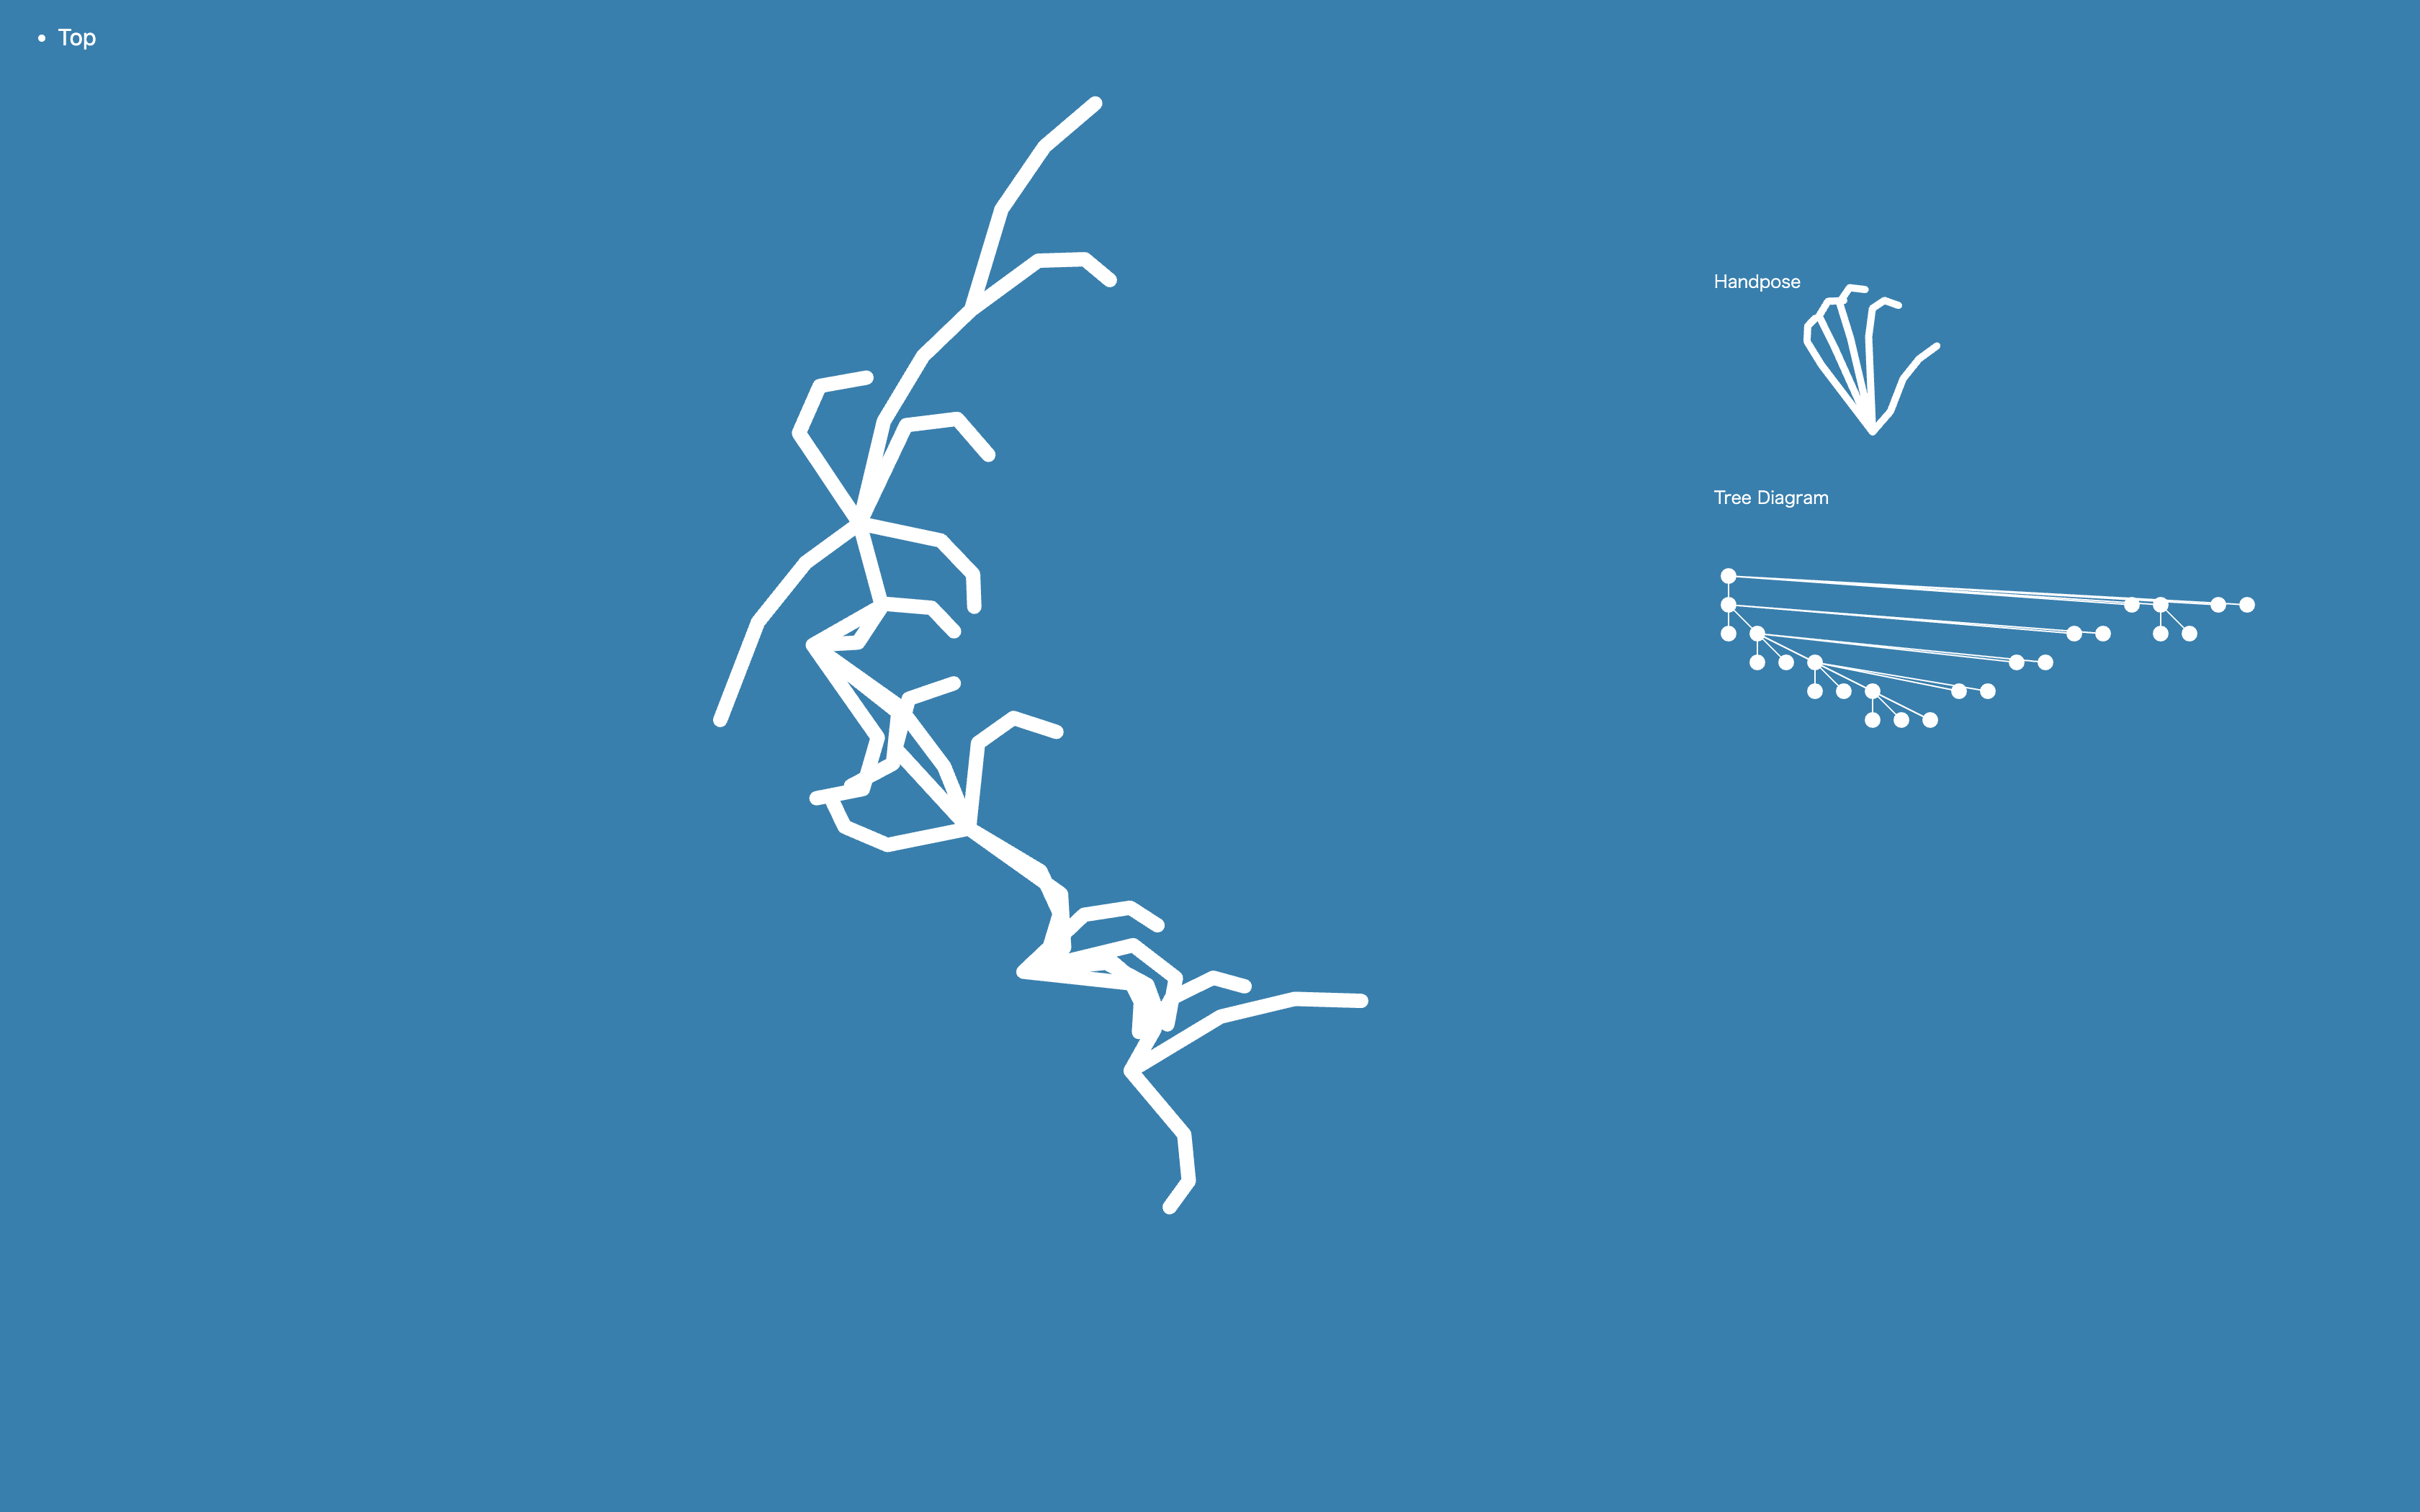
\includegraphics[keepaspectratio, width=7cm]{img/networked_finger.png}
    \caption{Networked Finger}
    \label{fig:networked_finger}
  \end{minipage}
  \begin{minipage}[b]{0.5\linewidth}
    \centering
    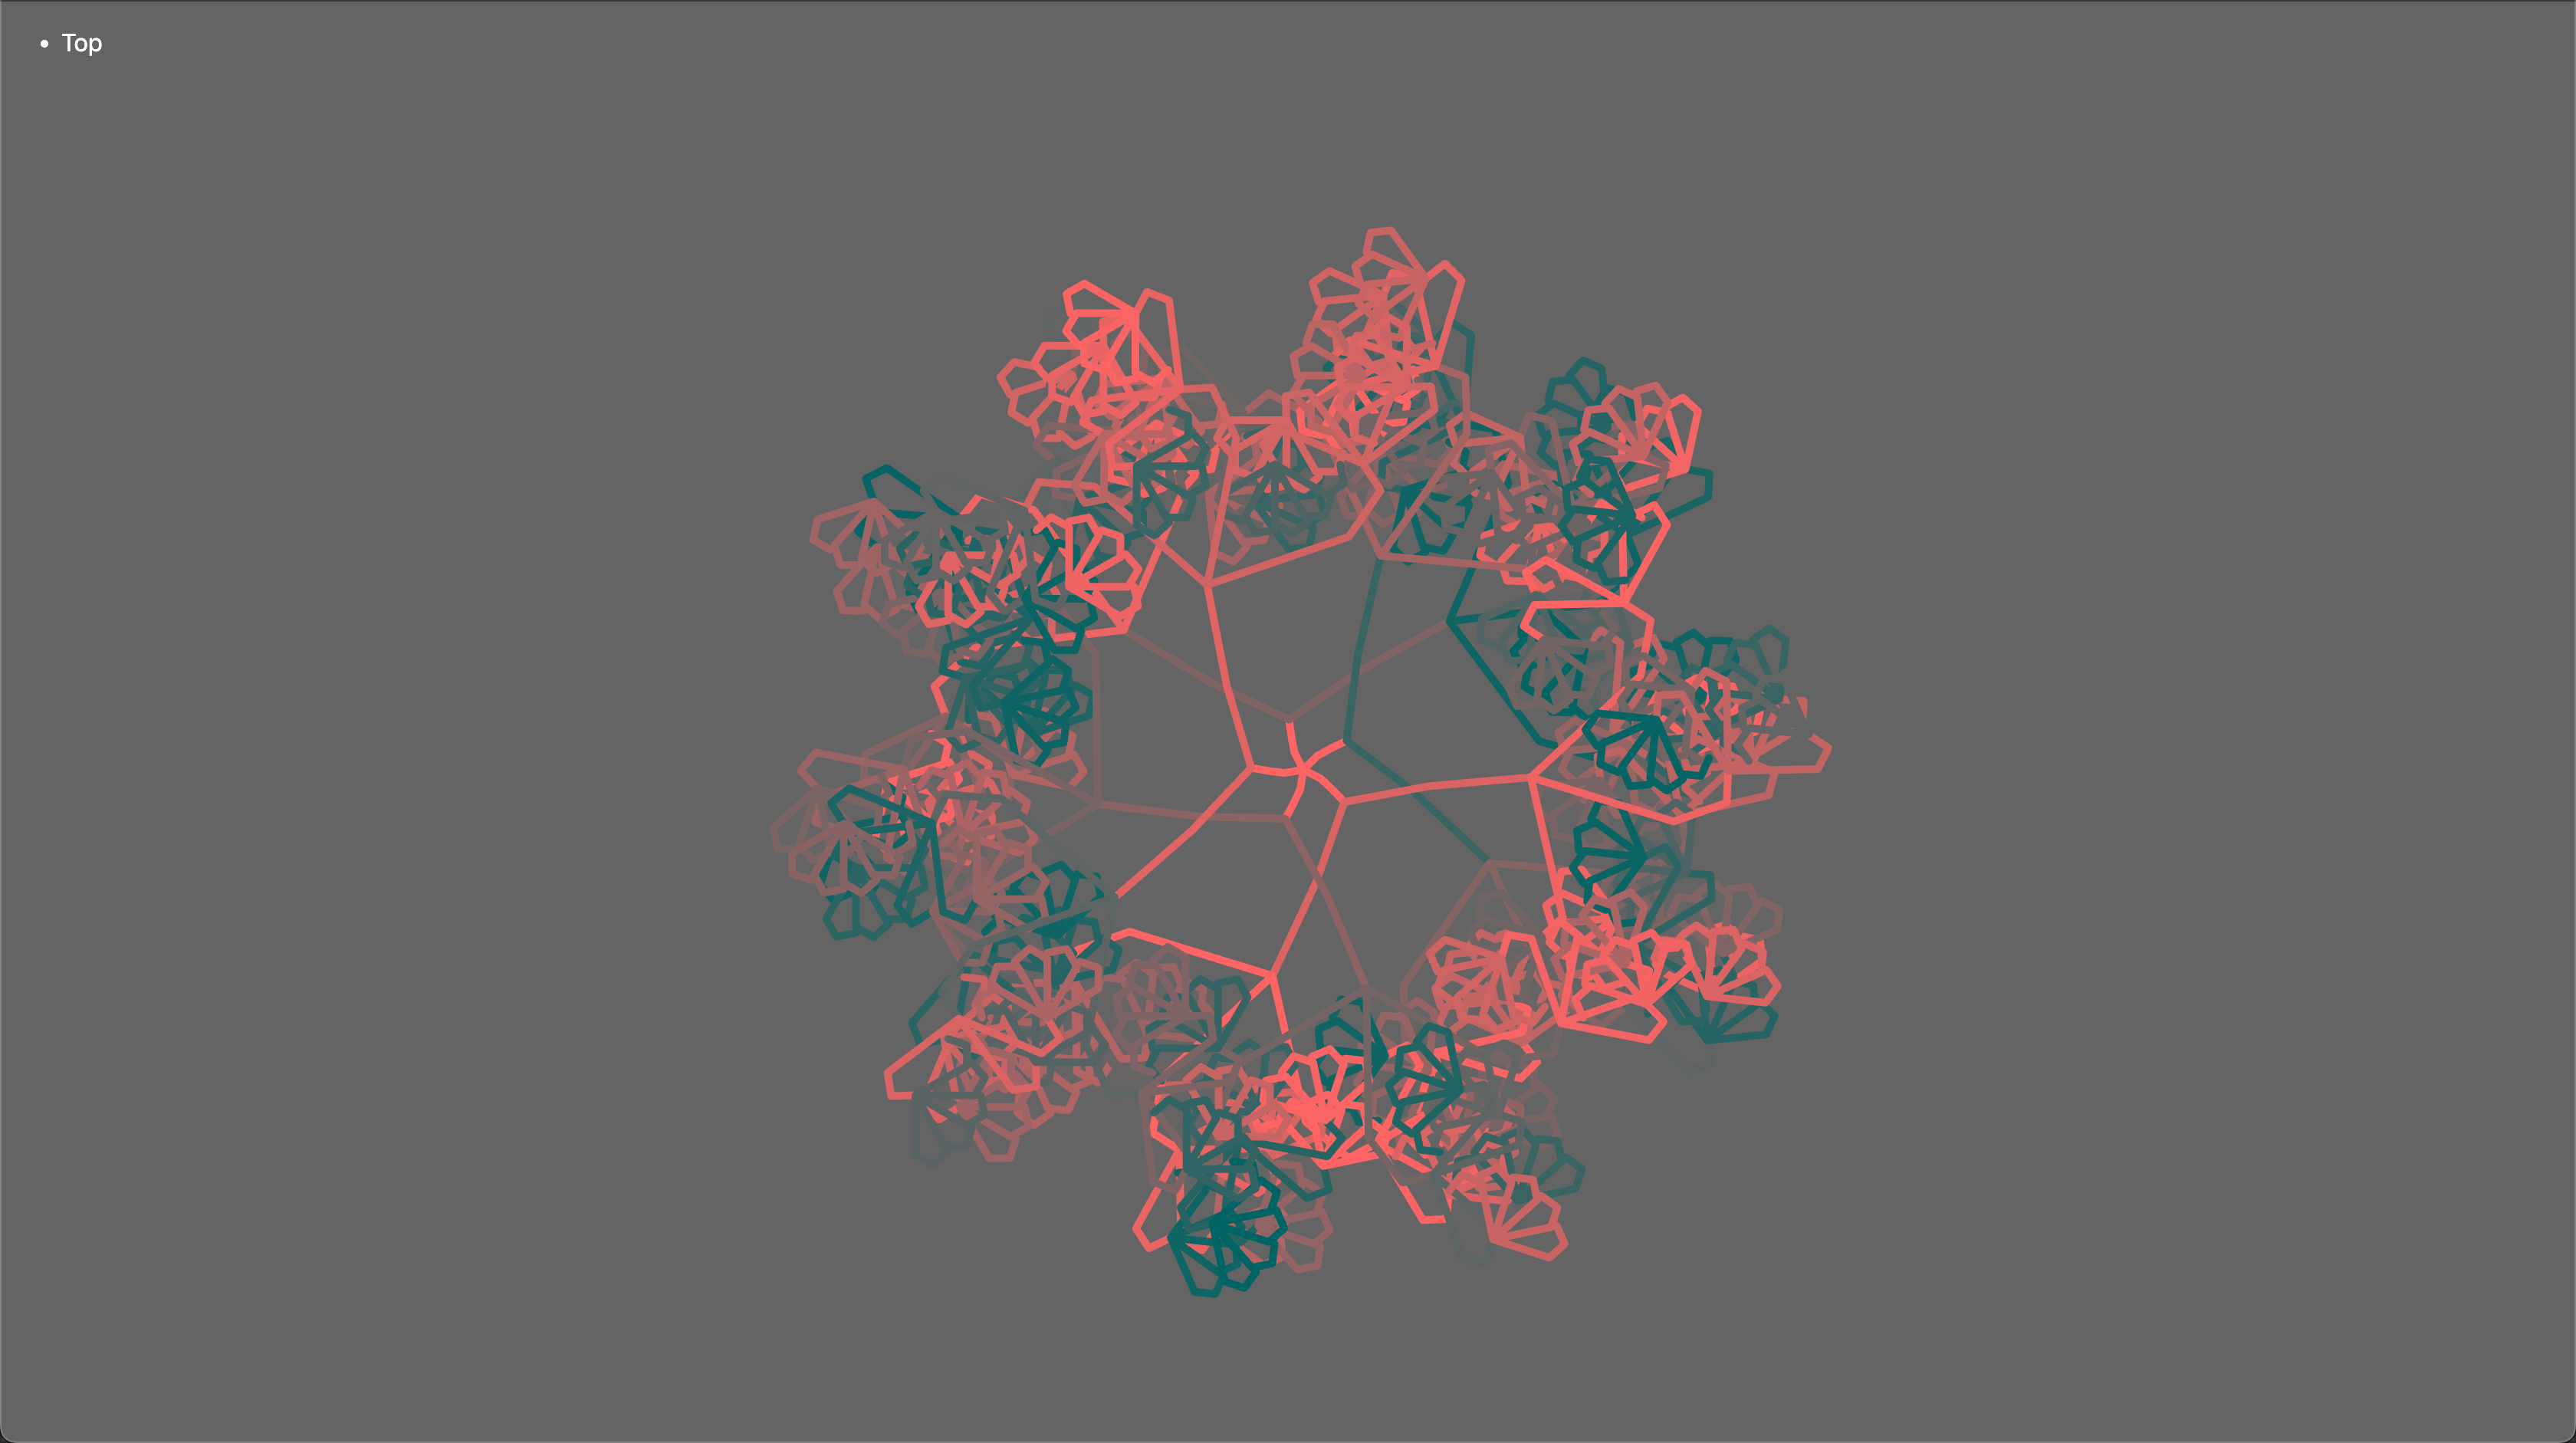
\includegraphics[keepaspectratio, width=7cm]{img/fractel_finger.png}
    \caption{Fractal Finger}
    \label{fig:fractal_finger}
  \end{minipage}
\end{figure}

\subsection{時間操作}
以下は、現在の自分の動きだけを表示するのではなく、過去の動きも表示するバリエーションである。図\ref{fig:prototype_delay}に示すプロトタイプでは、5本の指の動きが等間隔に並べられているが、それぞれの指は、鉛直上向きの角度に現在の指の動き、そこから時計回りに、順次過去の指の動きが並べられている\footnote{\url{https://interaction005-moe5dbh11-k1105.vercel.app/}}。このプロトタイプでは、指先を小さく動かすと、その動きが時計回りに伝播していくような動きが起こる。これは例えばゼリー状の物体を触れた時のような、物体の衝撃が全体へと伝播していくようすにも見立てられる。そのためか、柔らかいオブジェクトに触れているときのような手触りのようなものを感じた。
また、数ミリ秒前の動きが隣接する形に現れ、全体として2秒程の期間の全ての動きが表示されることになる。そのため、2秒間のあいだに動きの変化があれば、身体を動かしていても止まっていても画面に変化が現れることが、直感に反した動きとなることに注意が向く。

\begin{figure}[H]
  \centering
  
\includegraphics[width=15cm]{img/past_time.png}
  \caption{過去の動きを用いた例}
  \label{fig:prototype_delay}
\end{figure}

\subsection{ボール操作}
ここまでは手指をいかに変換するかについて探索を行なってきたが、その手指を用いた動きの複雑度に影響する要素としてボール操作について検討した。こうしたバリエーションを制作し、ボールがないものと並置して「IAMAS openhouse2023」にて展示した際、体験した方の一人から2つを比較して、手指の変換表現だけのものについては「途中から自分が何やってるか忘れてしまって、なんとなく指を動かすとなんとなく画面の描画内容が変わってる、となってしまっている」一方で「ボールの方はそんなことはなかった」とし、その理由として「具体的なタスクがあったほうがずっと続きやすい」といったことを挙げていた。そのため、よりタスクを明確化したバリエーションとして下記のような、マトあてのバリエーションも制作した。

\begin{figure}[H]
  \centering
  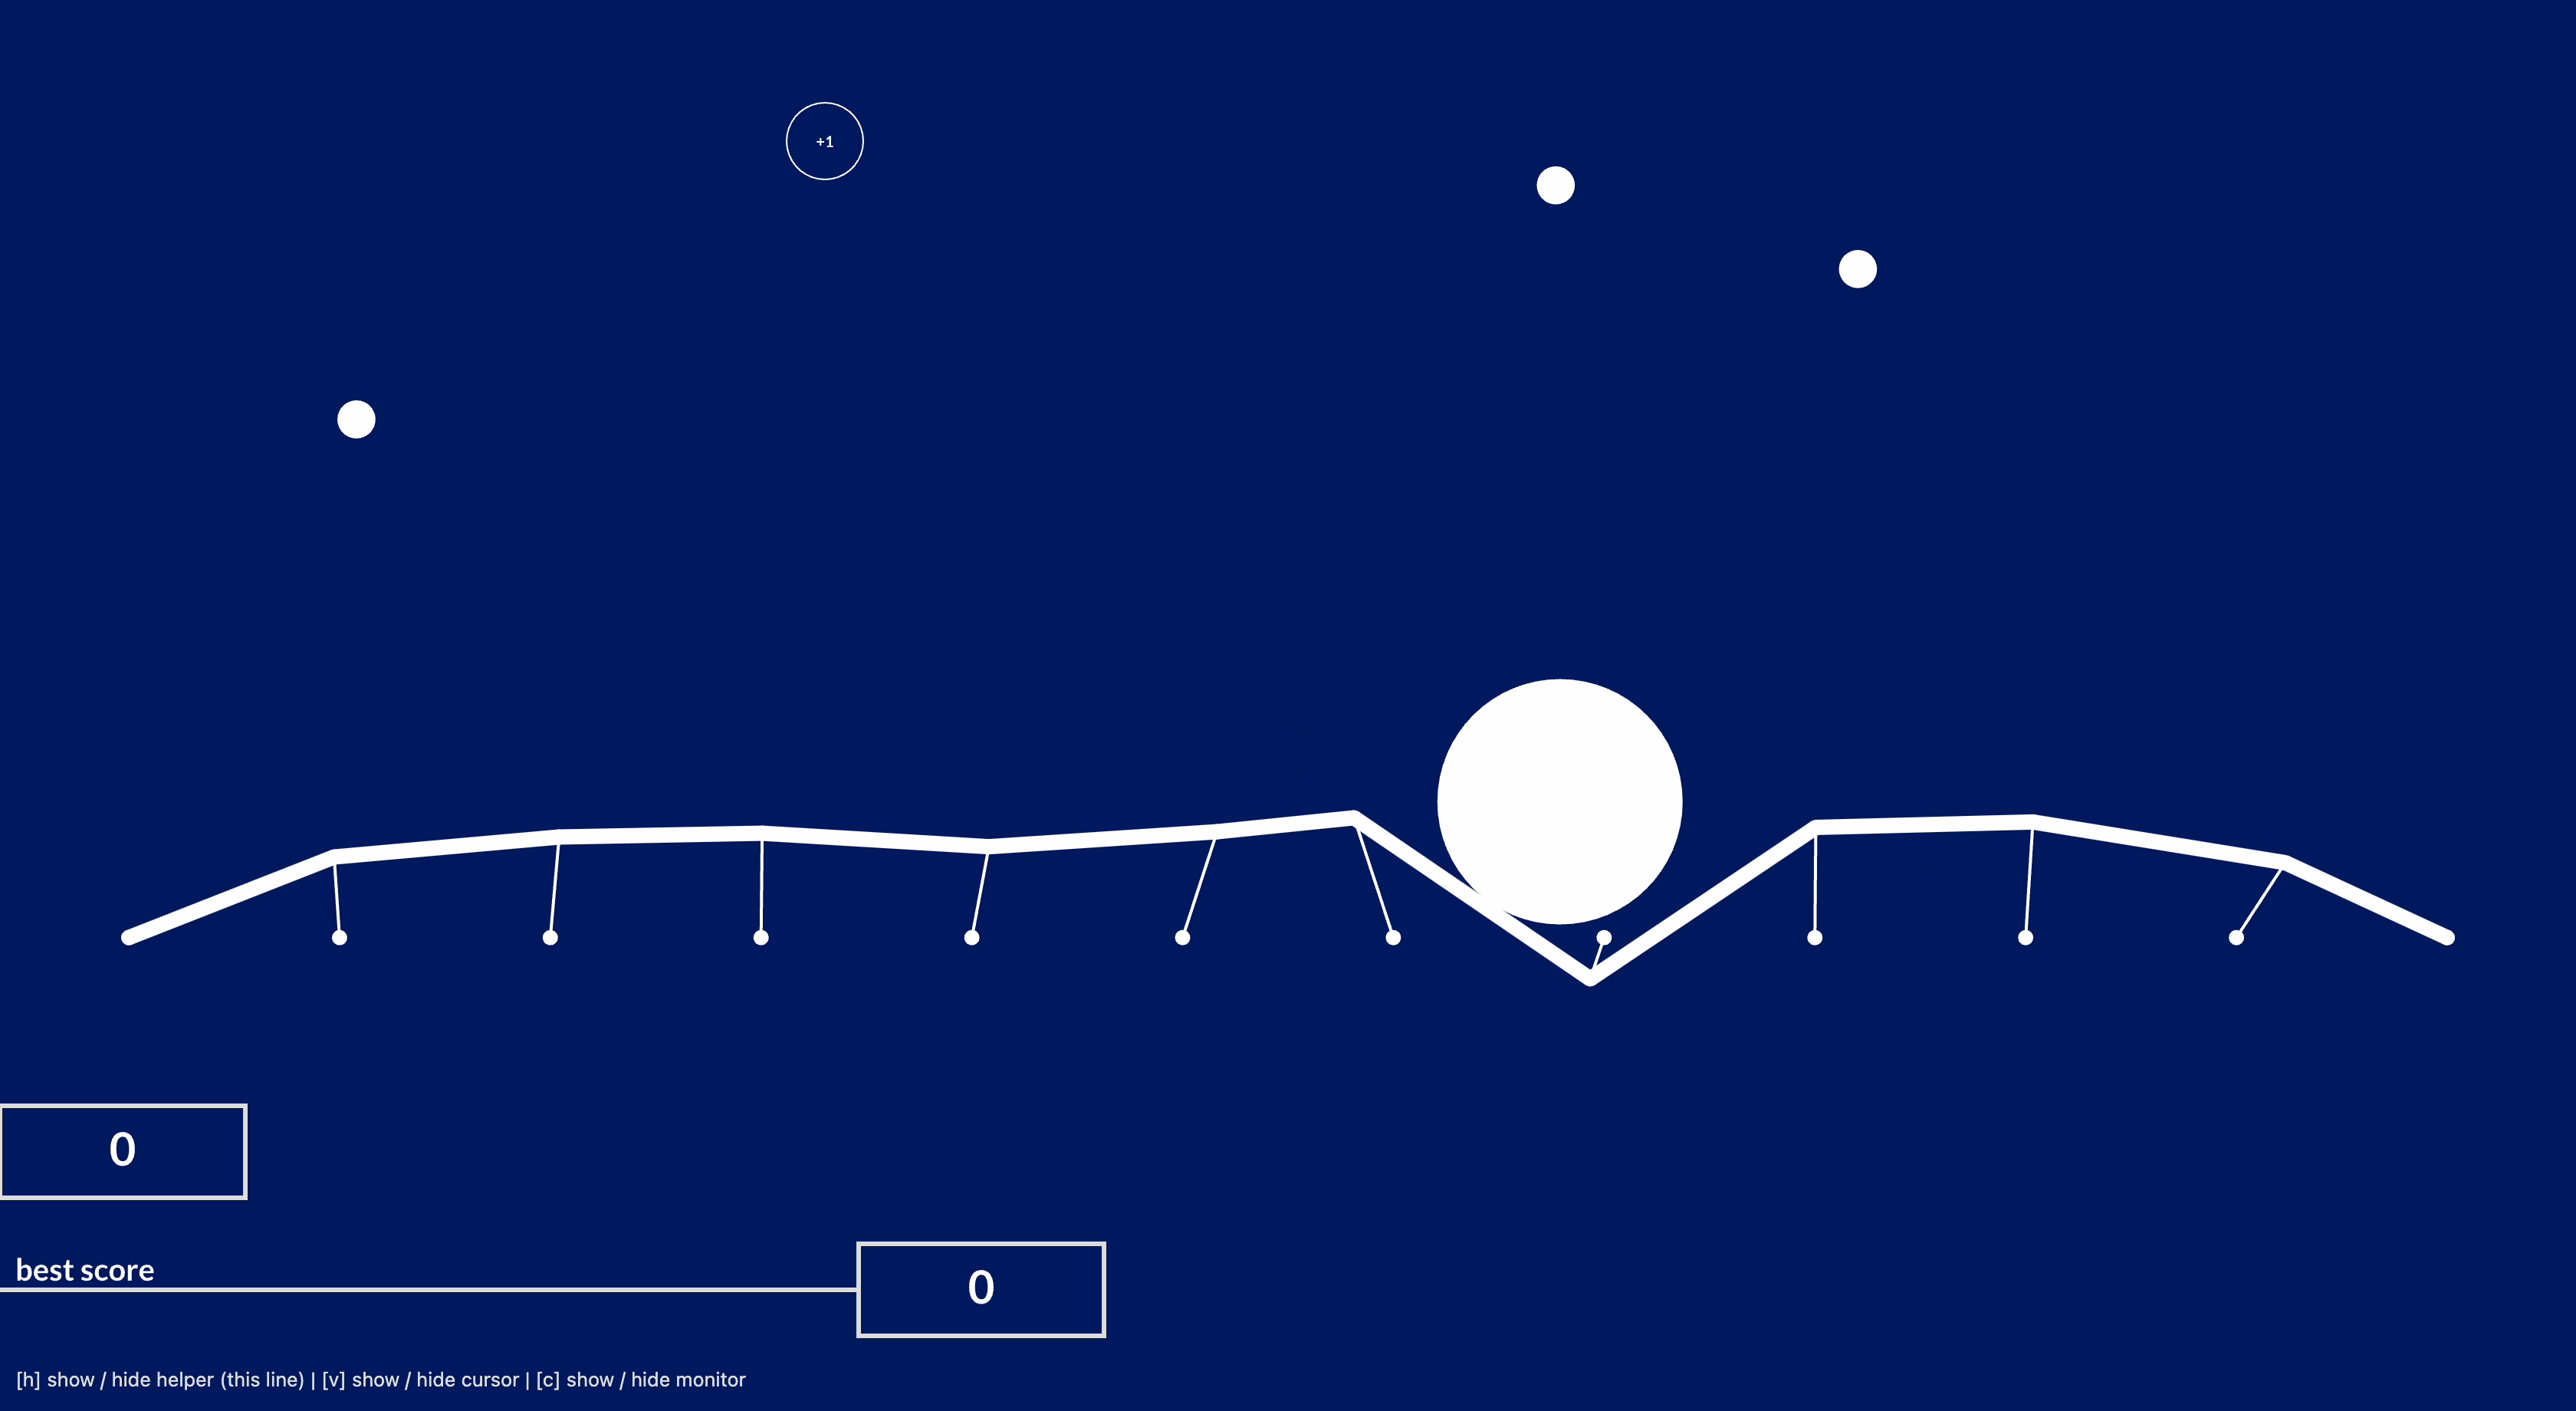
\includegraphics[width=15cm]{img/ball_overview.png}
  \caption{ボール操作の例}
  \label{fig:ball_overview}
\end{figure}

また、過去に制作したバリエーションを拡張する形で、ボール操作のパターンについて検討した\footnote{\url{https://interaction023.vercel.app/}, \url{https://interaction024.vercel.app/}}。

\begin{figure}[htbp]
  \begin{minipage}[b]{0.5\linewidth}
    \centering
    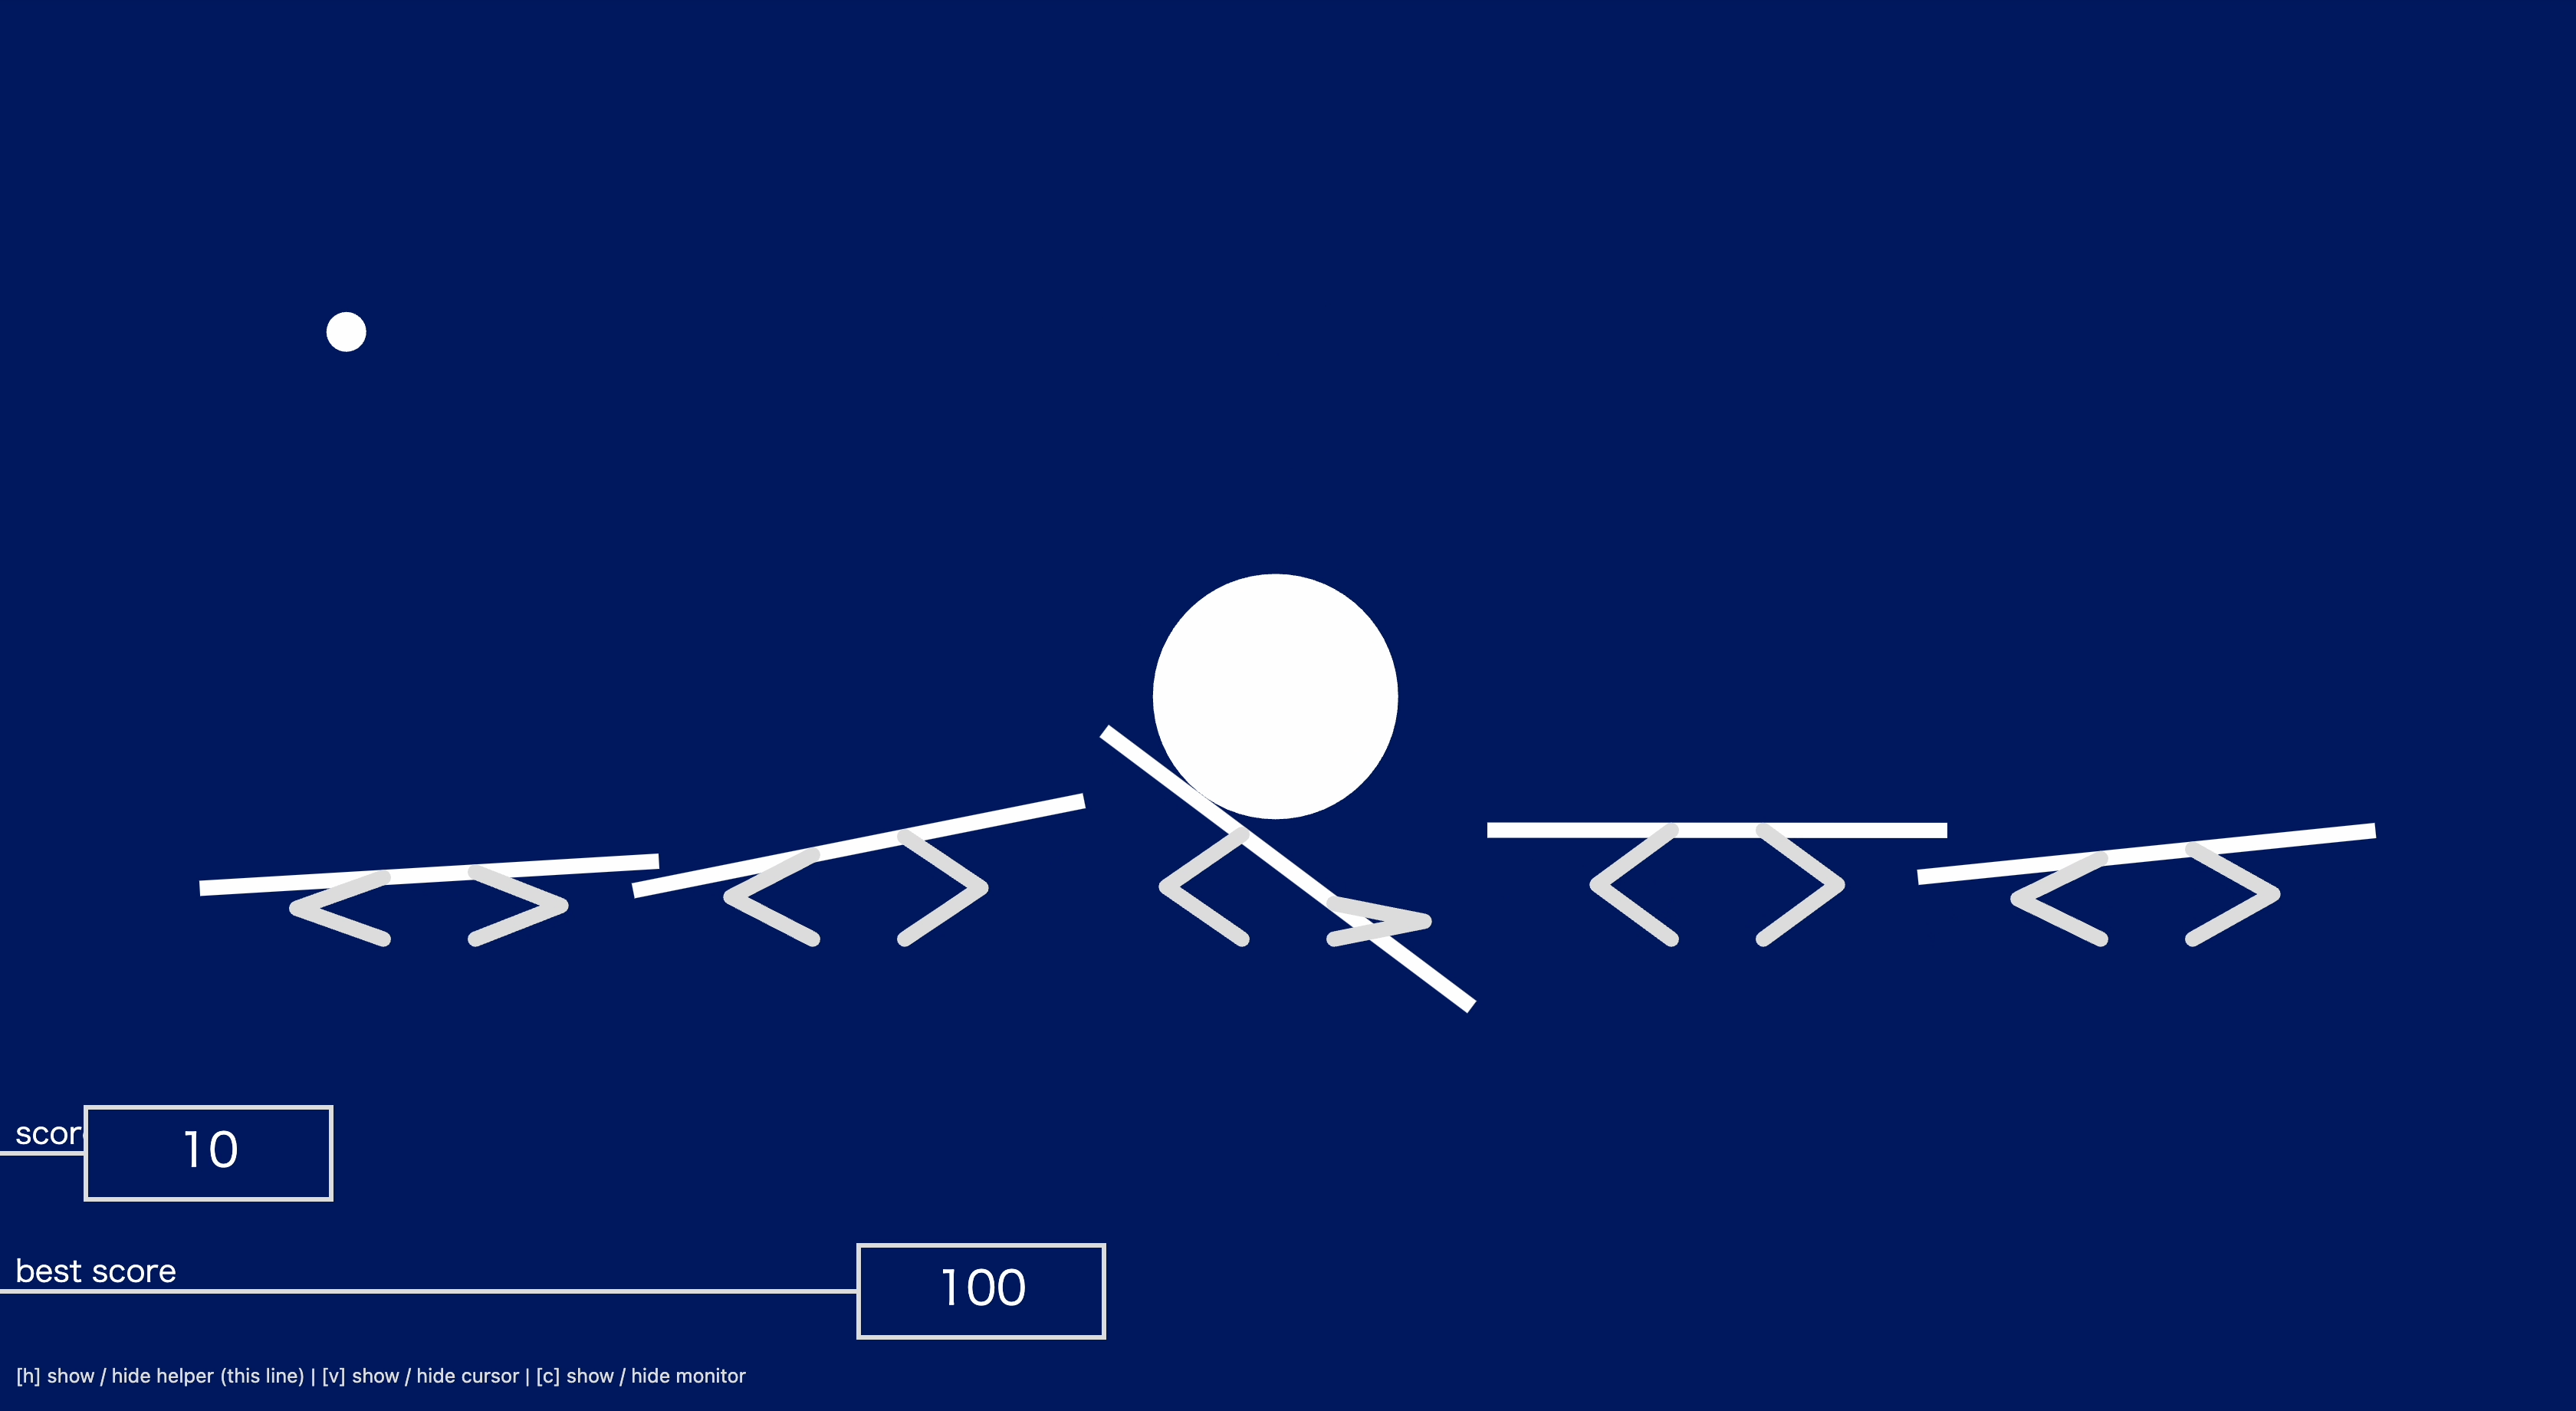
\includegraphics[keepaspectratio, width=7cm]{img/ball_0.png}
    \caption{「くの字」の並列配置を拡張したボール操作}
    \label{fig:ball_0}
  \end{minipage}
  \begin{minipage}[b]{0.5\linewidth}
    \centering
    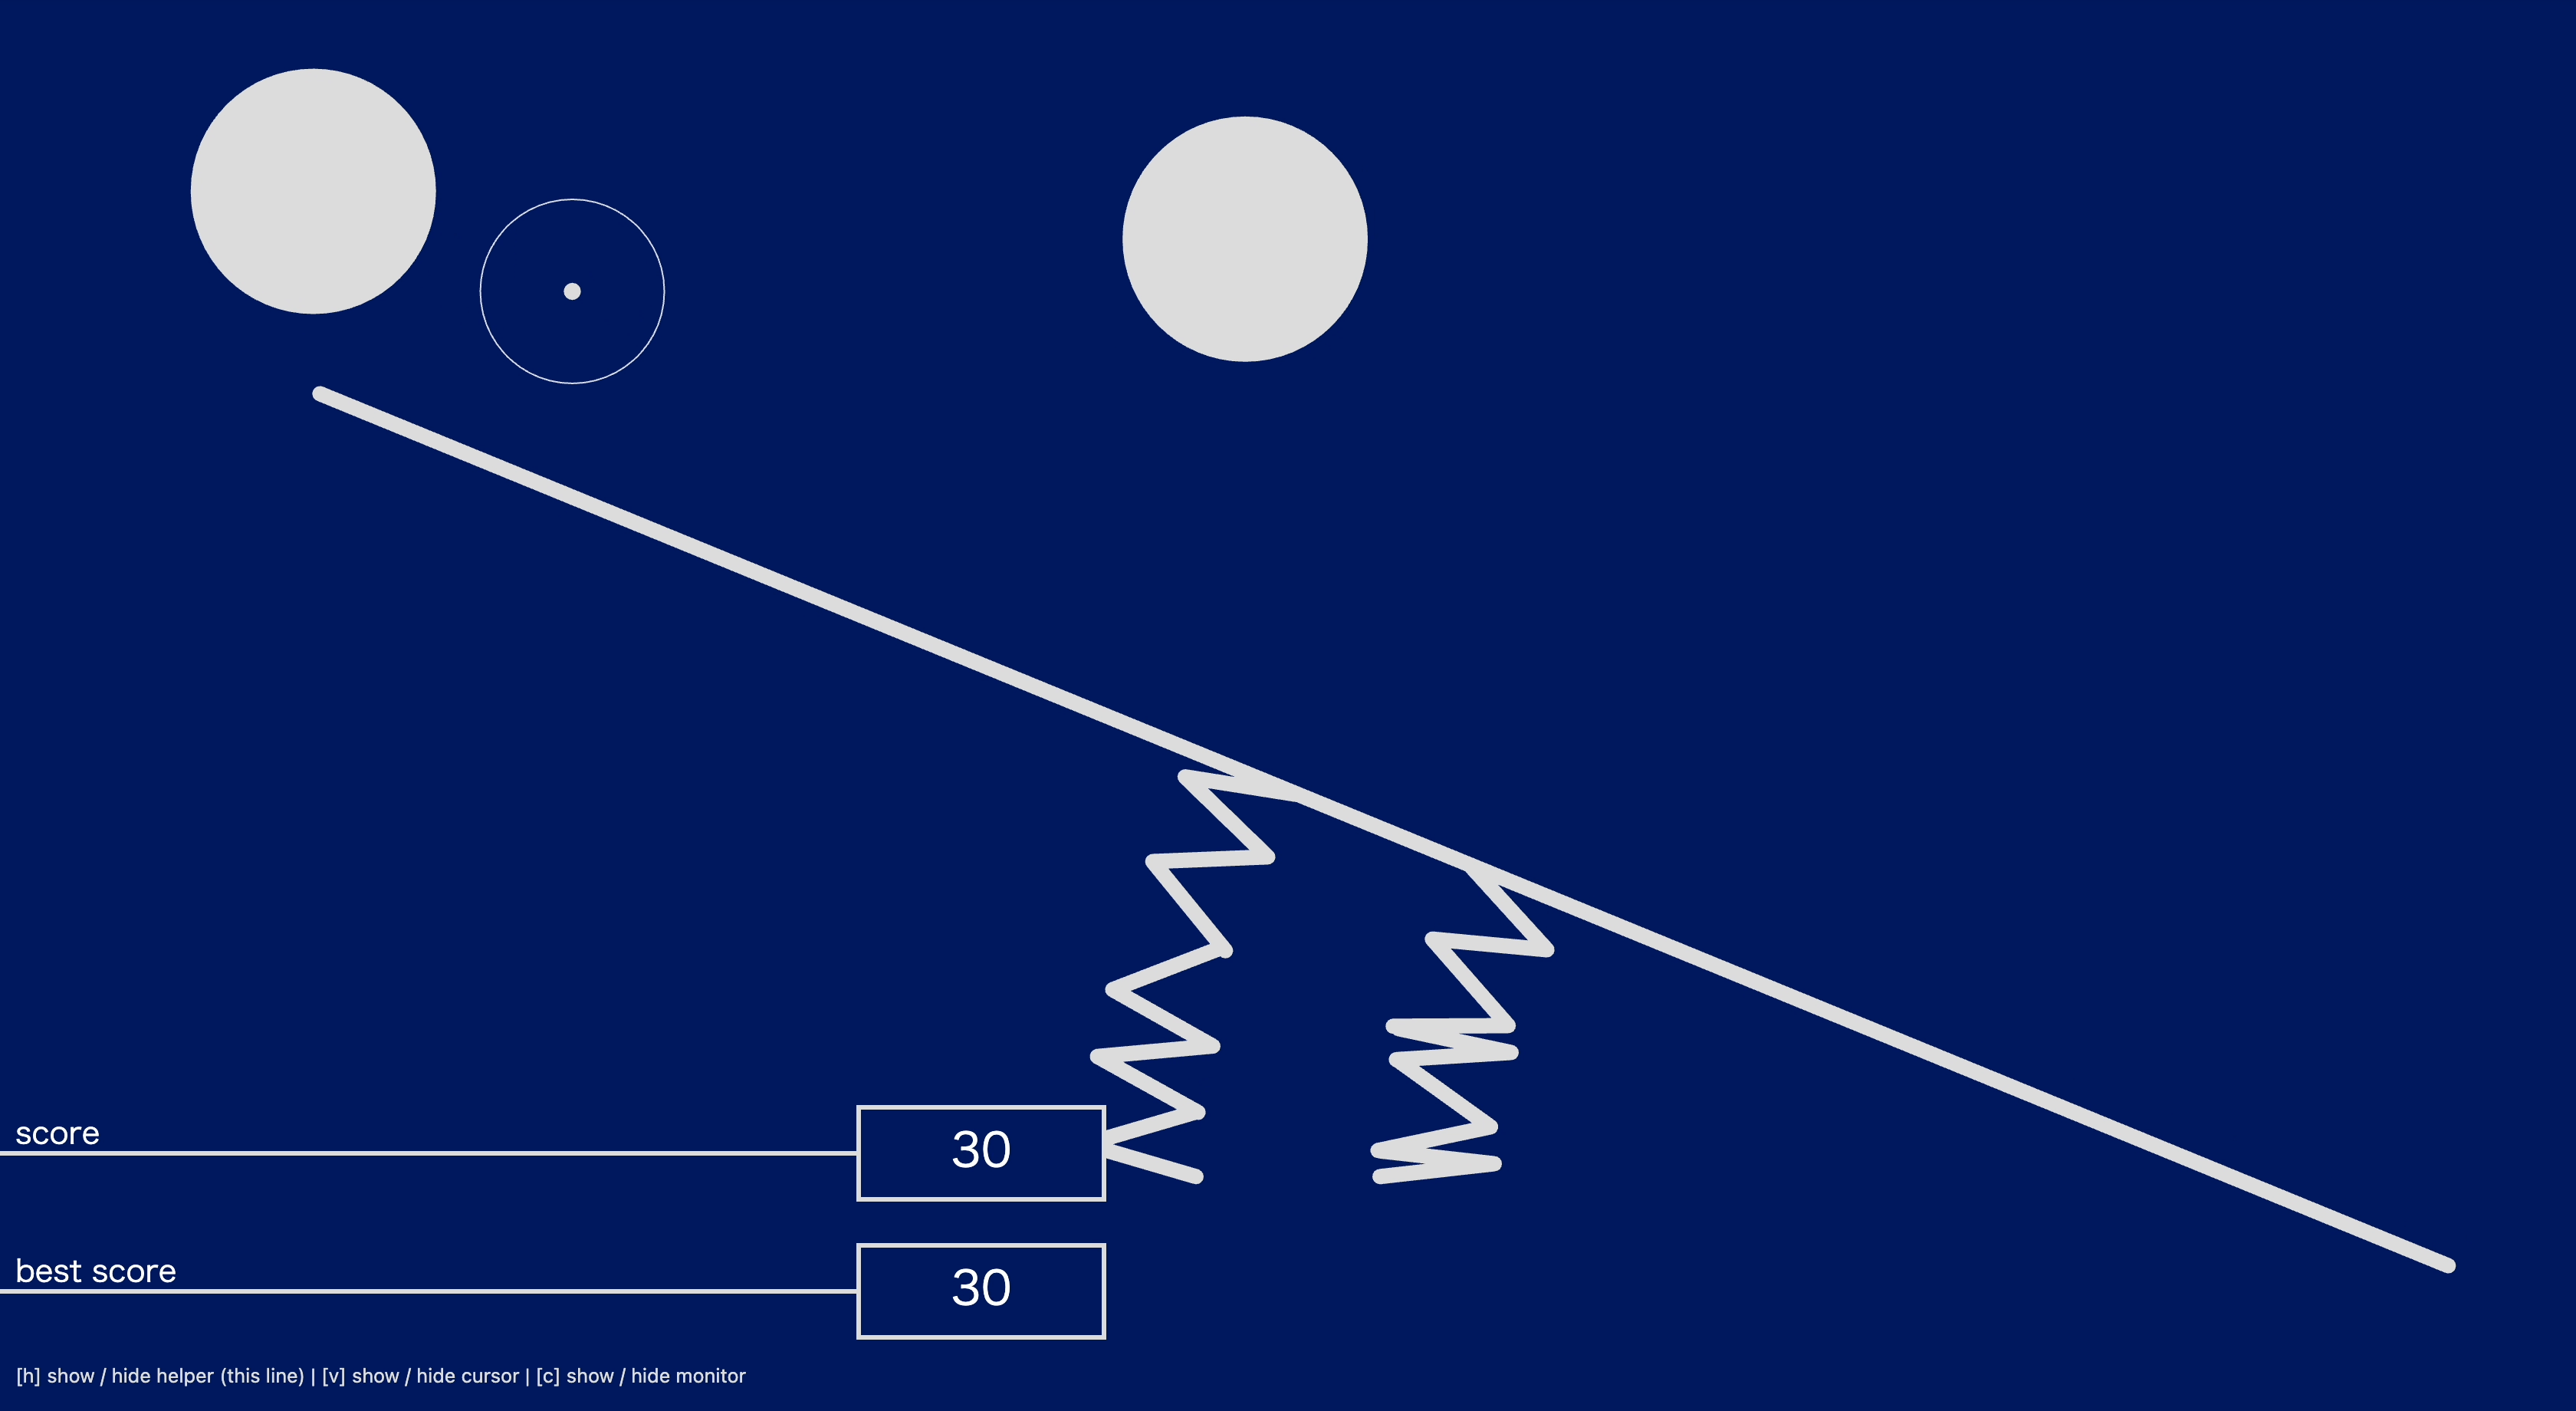
\includegraphics[keepaspectratio, width=7cm]{img/ball_1.png}
    \caption{「くの字」の直列連結を拡張したボール操作}
    \label{fig:ball_1}
  \end{minipage}
\end{figure}

\section{表現の選定}
ここまで、変換表現を扱ったプロトタイプについて概観してきた。以下では、これらのプロトタイプを踏まえて、「人馬一体感」の生起に向け、それを具現化する表現とは何か、という観点から重要だと考えられる観点を列挙し、プロトタイピングについて分析する。

\subsection{自分が動かしている感覚が強い表現}
1つ目の観点として、手指の微細かつ複雑な動きをもって、緻密な制御をしているという感覚が引き出される表現へと絞り込んでいくことにした。これは\ref{prototyping_concept_making}節で述べたように、手指の変換表現における快体験の一つであり、またこの構造に合わせて動かすようになったときに、強く一体感を喚起すると考えたためである。

形状については、指を単位としない場合についても検討したが、指は一本一本独立して動かすことができる性質上、指が一つの単位となっている変換に注意を向けやすいのではないかと考えた。その中でも、円形、くの字、ドットなどの変換を試みたが、動きに対して注意が向けられたのは「くの字」の形状であると感じられた。この理由について、身体動作である指の屈曲との対応から考察する。指の屈曲が円の半径へと対応している場合と「くの字」のような折り曲げ動作に対応している場合とを比べたとき、後者の方が指の屈曲の運動との類似性が高い。そのため、探索的に手指を動かす中で、手指の屈曲の動きとのリンクを見出した時にぴたりと一体感が感じられるような感覚があるのではないだろうか。他方で、円の半径に関節の動きをマッピングさせるような表現については、手指の運動が収縮の動きに変換しているため、どのような動きをとっても先のような一体感を感じづらいのではないかと考えた。

% これは、Gallagherの「運動主体感(sense of agency)」\cite{Gallagher2000}の誘起に関与する「感覚運動手がかり」の効果ではないかと考えられる。感覚運動手がかりとは、運動から得られる感覚フィードバックとその内的予想との予測誤差を表すもので、この誤差が小さいときに「まさに自分が動かしている」という感覚(運動主体感)が誘起されるという\cite{miyawaki}。


マッピングに関しては、1つの指の動きが規則的に配置される場合について、構造としての複雑度が上がっているにも関わらず、体感として複雑度が上がったようには感じられなかった。これについては、グラフィックデザイナーの女性が体験した際、「構造としては緻密であるのに、動きは単純であるように感じる」と意見したことにも重なる。その理由として彼女は、「対称性が前面に出ているため、シンボルとしての印象を強く感じてしまう」「意識していないところも同時に動いている感覚があるため、自分の動きだと思えない」からではないかと推測した。
この「意識しないところも同時に動いている感覚」は、1つの指の動きを複数の箇所に対応させる構造が持つ問題点のように思われるが、一方で1つの動きが分散して不規則に配置される図\ref{fig:networked_finger}のような形状の場合は、1つの動きが複製されていても、指の数が増えると複雑度も比例して上がっているように感じられた。これは、全体が秩序だった構造をしておらず、指一本一本の動きの組み合わせから生じる総体の形状について、予測がつきづらく、また記憶に留めておくことも難しい「行きつ戻りつ」な感覚があるためではないかと推測した。

こうした分析から、「自分で動かしている感覚」について、次のようなものは相応しくないと判断した。一つは、円の収縮運動といった身体動作との関わりが薄いもの、またもう一つは「シンボルとしての印象」が全景化する、規則的かつ一つの動きが複数に配置されたようなパターンである。

\subsection{目的意識の創発}
また、体験の中で目的意識を誘発するような表現に注目した。ここでの「目的」とは、高い自由度と複雑度のある空間の中でプレイヤーが定義する、サンドボックスゲームに見られるような「創発」によるものである。「目的の創発」に着目した理由は、その対極にある明示的な目的が設定された状態だと、探索的な試行が減り、インタラクションを通した唯一性のある関係が芽生えづらいのではないかと考えたためである。
中でもボールの出現は、手の変換だけの表現とは異なる複雑度があり、「変換された手とボール」の関係だけで様々な体験の質が創発するのではないかと考えた。また、ボールという直接的に動かすことのできる対象ではないものが現れたことによって、「確認」のような探索的な身体動作のみならず、それをいかに器用に扱えるかといった、巧みさに関する試行錯誤の可能性が生じた。特に、マトに当てることを目指す中では、特に巧みさが重要となる。ただし、プロトタイピングの過程で取り入れていた「スコア」の表記は、「目的の創発」を阻害するものであるとして、最終的には採用しなかった。スコアが存在することで「マトに当てる」という目的意識を強く与えてしまうことが挙げられる。強固な目的意識の設計は、より多くの人を同一の目的に向かわせ、その目的以外の興味や注意が生じる余地が損なわれると考えた。

\subsection{注意の対象による作品の分割}
ボール操作に関するバリエーションを制作した際の気づきから、ボール操作は「もどかしさ」を経験するほどの比較的強い注意を喚起する一方で、ボールがなかった場合と比べると、注意の向く対象が、手指の運動ではなく、ボールと手指の関係性に注意が生じることがわかった。そこで、最終的な作品としてはその2つを分けて構成した。そして、手指の形状が変化することを起点に注意が生じる作品と、ボールと手指との関係性に注意が生じる作品というように、何に注意が生じるかという観点に着目して2つの体験を整理した。

\subsection{モーフィングの追加}
過去に展示していたバージョンではモーフィングを示さず、手指が認識されたとたんに変換された状態の手指が提示される作品形態であった。しかし、全く見慣れない形なので「手指を細かく動かせる」といった、作品がもつ可能性に気づけないことがある。そこで、形状の変化を確認できるモーフィングを実装した。そうすることで、白い点が関節を表していること、そして手指の運動を細かくトラッキングしていることを事前に伝え、それが形を変えた姿として画面の前に提示されていることがわかるようになる。こうすることで、手指の構造から離れていくことを認識することがきっかけとなって違和感を誘発でき、一番最初の意識的な身体動作を喚起するきっかけとなるのではないかと考えた。

\section{展示形態の設計}
展示形態について、時系列順に過去2つのバージョンについて説明し、その流れから最終的な展示形態の根拠を示す。

\textbf{初期:カメラを画面前に配置した状態}\\
最初期は、体験装置について下図\ref{fig:kyotai_ver0}のように、モデルトラッキングを行っているカメラを直接画面の前に配置していた。
\begin{figure}[H]
  \centering
  \includegraphics[width=12cm]{img/kyotai_ver0.jpg}
  \caption{初期:カメラを画面前に配置した状態}
  \label{fig:kyotai_ver0}
\end{figure}

プロトタイピングの段階でもあったため最低限の構成としていたが、この構成には次のような問題があった。
\begin{quote}
  \begin{itemize}
    \item カメラのトラッキング精度が環境光の影響を受けて変動してしまう
    \item 体験者ではない周囲の人の手指を間違ってトラッキングしてしまう
    \item 手指の形がそのまま出力されるわけではないので、トラッキングの範囲がわからず、腕を大きく振ったり、手指がトラッキングできない範囲で動かしてしまう
  \end{itemize}
\end{quote}

このため、制作者が指示をすることなく自由に体験してもらうことを意図していた展示であっても、体験方法がわからなかったり、後方で見守る人の手を誤ってトラッキングしてしまうといった問題が起き、有効なフィードバックを得ることができなかった。

\textbf{中期:専用筐体を用いて手首を固定した状態}\\
こうした課題を踏まえて、次に専用筐体を制作し、穴に手を入れる形式について試した(図\ref{fig:kyotai_ver1})。

\begin{figure}[H]
  \centering
  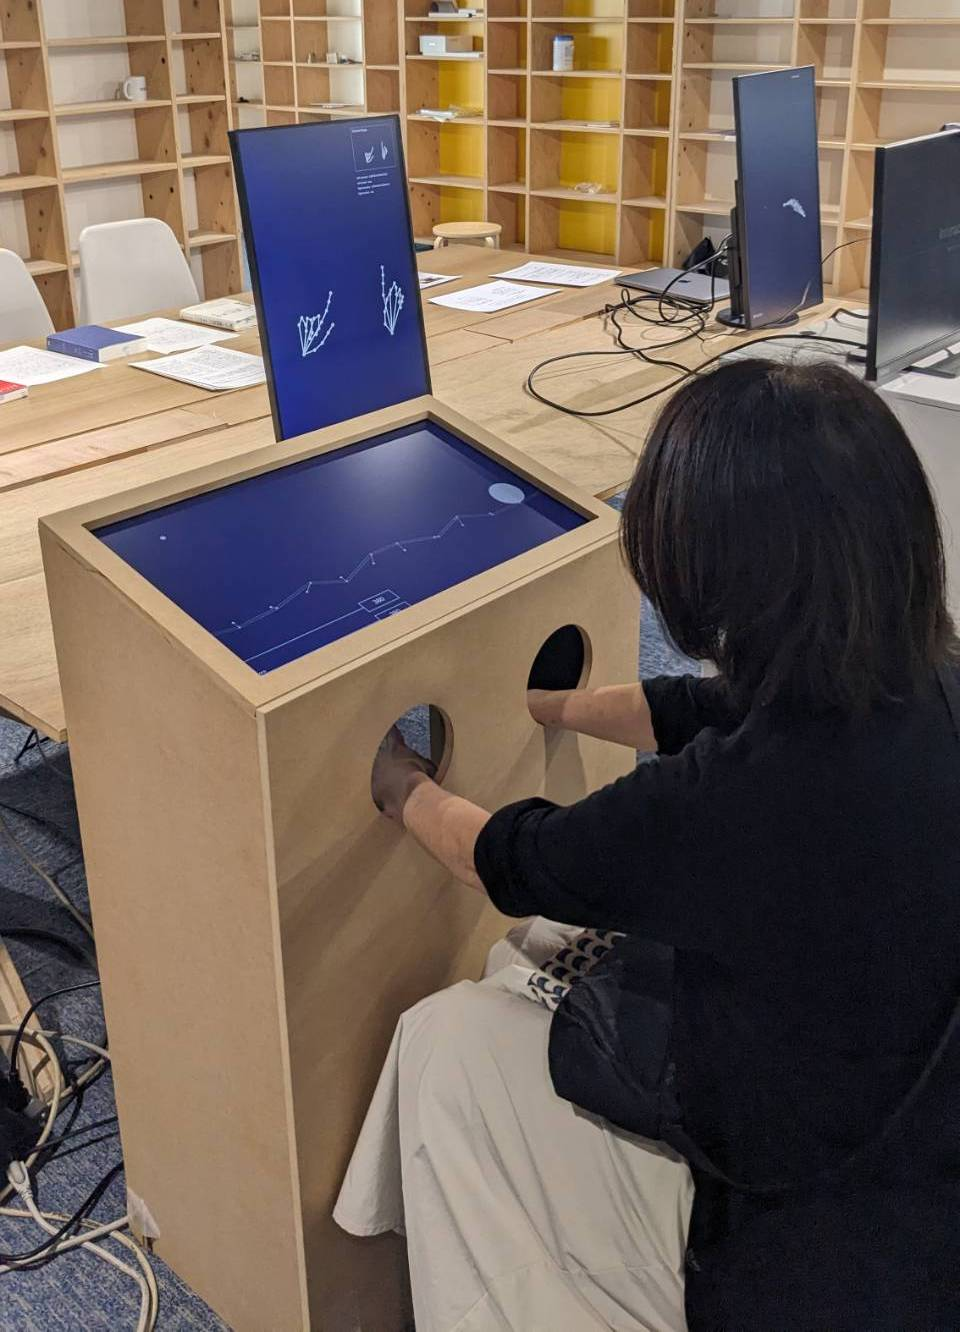
\includegraphics[width=8cm]{img/kyotai_ver1.jpg}
  \caption{中期:専用筐体を使用してカメラを隠蔽した状態}
  \label{fig:kyotai_ver1}
\end{figure}

この形式では、カメラの画角に映り込むのは筐体の内部と体験者の手のみであるため、環境光の影響や周囲の人の影響を受けずに体験できるようになった。また、穴によって手首の位置が固定されるため、腕を大きく振ることが構造上不可能となり、比較的身体動作の幅が抑えられた。

ただし、この形式は単に上記の問題を解決したというだけではなく、指先の動きが見えなくなったこと、画面に対する指先の位置関係についてを変更するものであった。

画面に対する手指の位置関係については、本作品では手指の形状が、もとの形とは全く関係のない構造へと変化するため、作品体験には大きな影響はないと判断した。手指の動きが見えなくなったことについては、画面の中の手指は体験時、自身の身体に代わる存在であるから、同時に視認できない今の形態の方がむしろ、より適した構成であると判断した。

しかしその一方で、手首の動きを固定してしまったことは、身体の動きを過剰に限定してしまう結果となった。身体の動きを限定してしまうと、何か特定の動作を求められているような説明的な構成になってしまう。そのため筐体としては、より簡素な構成が好ましいと判断した。


\textbf{作品展示:専用筐体を用いて手首を固定せず指先を自由にした状態}\\
そこで最終的には、図\ref{fig:kyotai_ver2}のような、トラッキングの範囲を暗示しながら、手首を固定しない方式に変更した。また、トラッキングに用いるカメラを、視野角150°の広角カメラ(Sanwa Supply CMS-V43BK-3)に変更し、大きく手指を動かしてもトラッキングの外れることの少ないものへと変更した。

\begin{figure}[H]
  \centering
  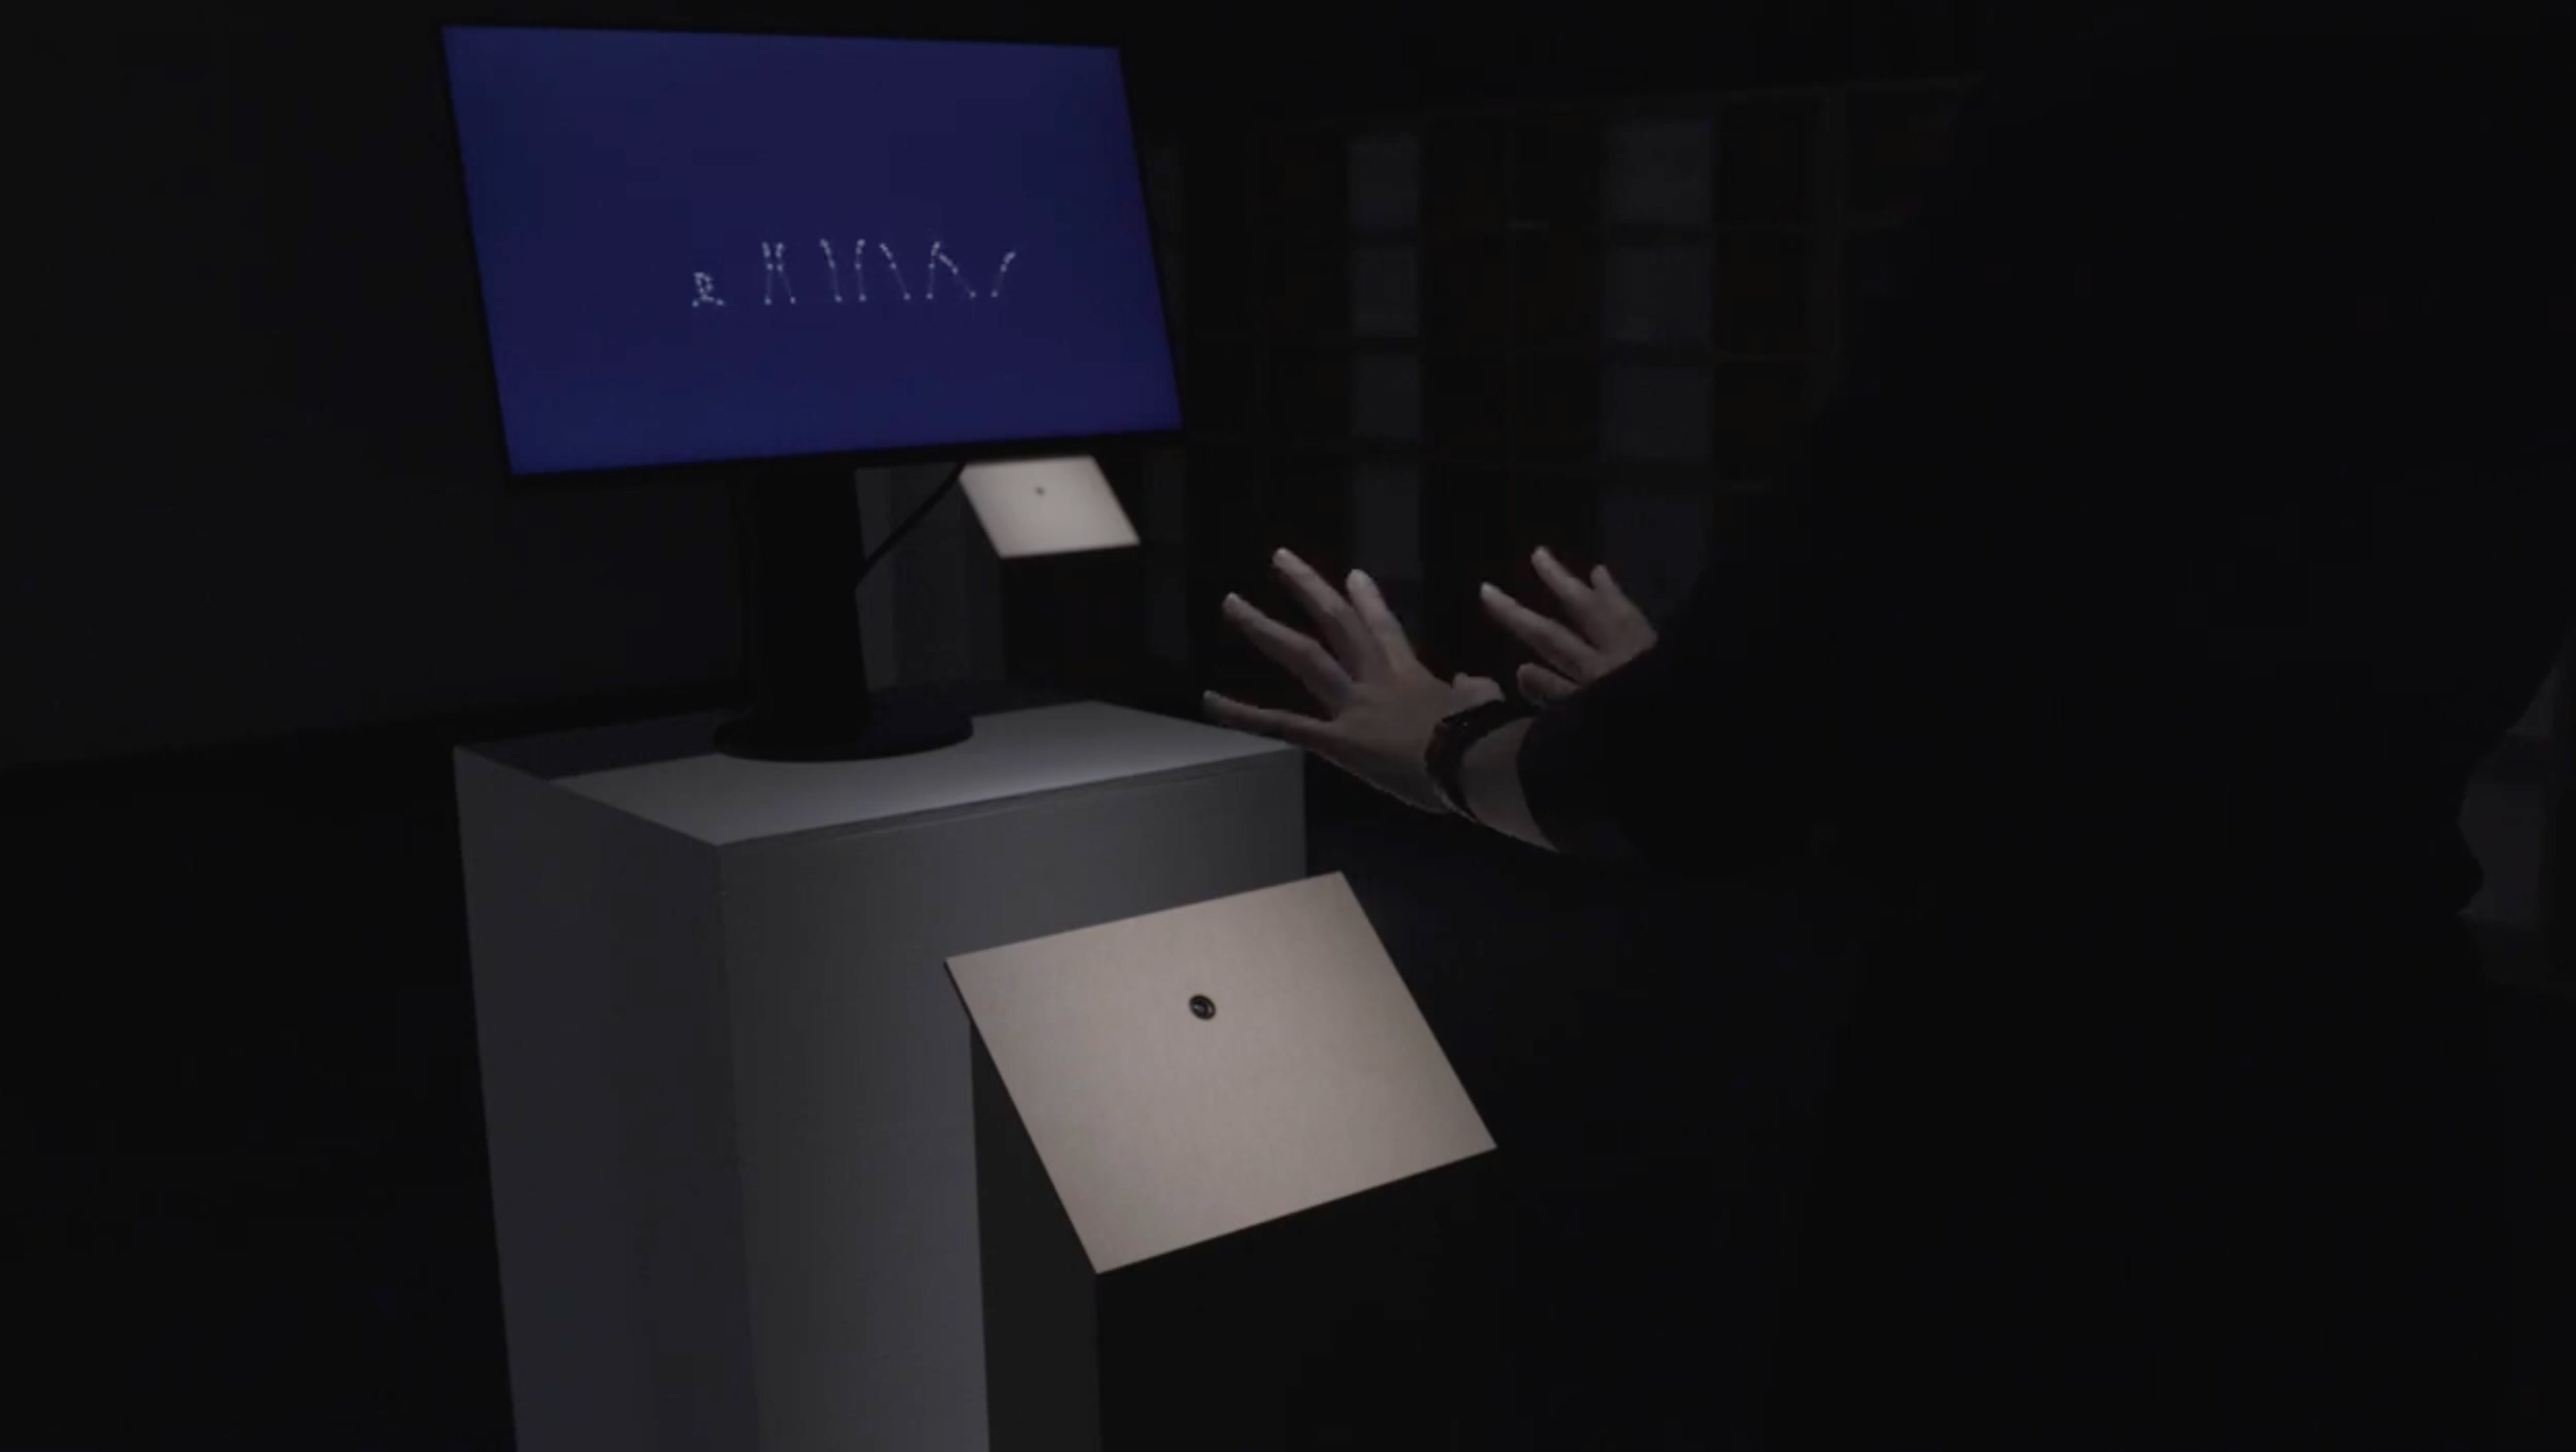
\includegraphics[width=12cm]{img/kyotai_ver2.png}
  \caption{作品展示の際の筐体}
  \label{fig:kyotai_ver2}
\end{figure}

筐体の高さは腰ほどの高さ(850mm)とすることで、キーボードのブラインドタッチのように、画面を見ながら手を同時に見ることが難しい構成とした。

カメラは、鉛直上向ではなく斜めを向いているので、筐体の前に立つと体験者の身体と手指の位置が重なり、トラッキングしやすい状況ができる。

また、ライティングの調整によってトラッキングの精度を高めた。
最終的な展示形態では、スポットライトを当てることで筐体周りを明るくすると同時に照り返しで手元の採光をし、周囲の照明を落とすことで明暗差を作ることで、手指の姿勢を認識しやすくなる。

\begin{figure}[H]
  \centering
  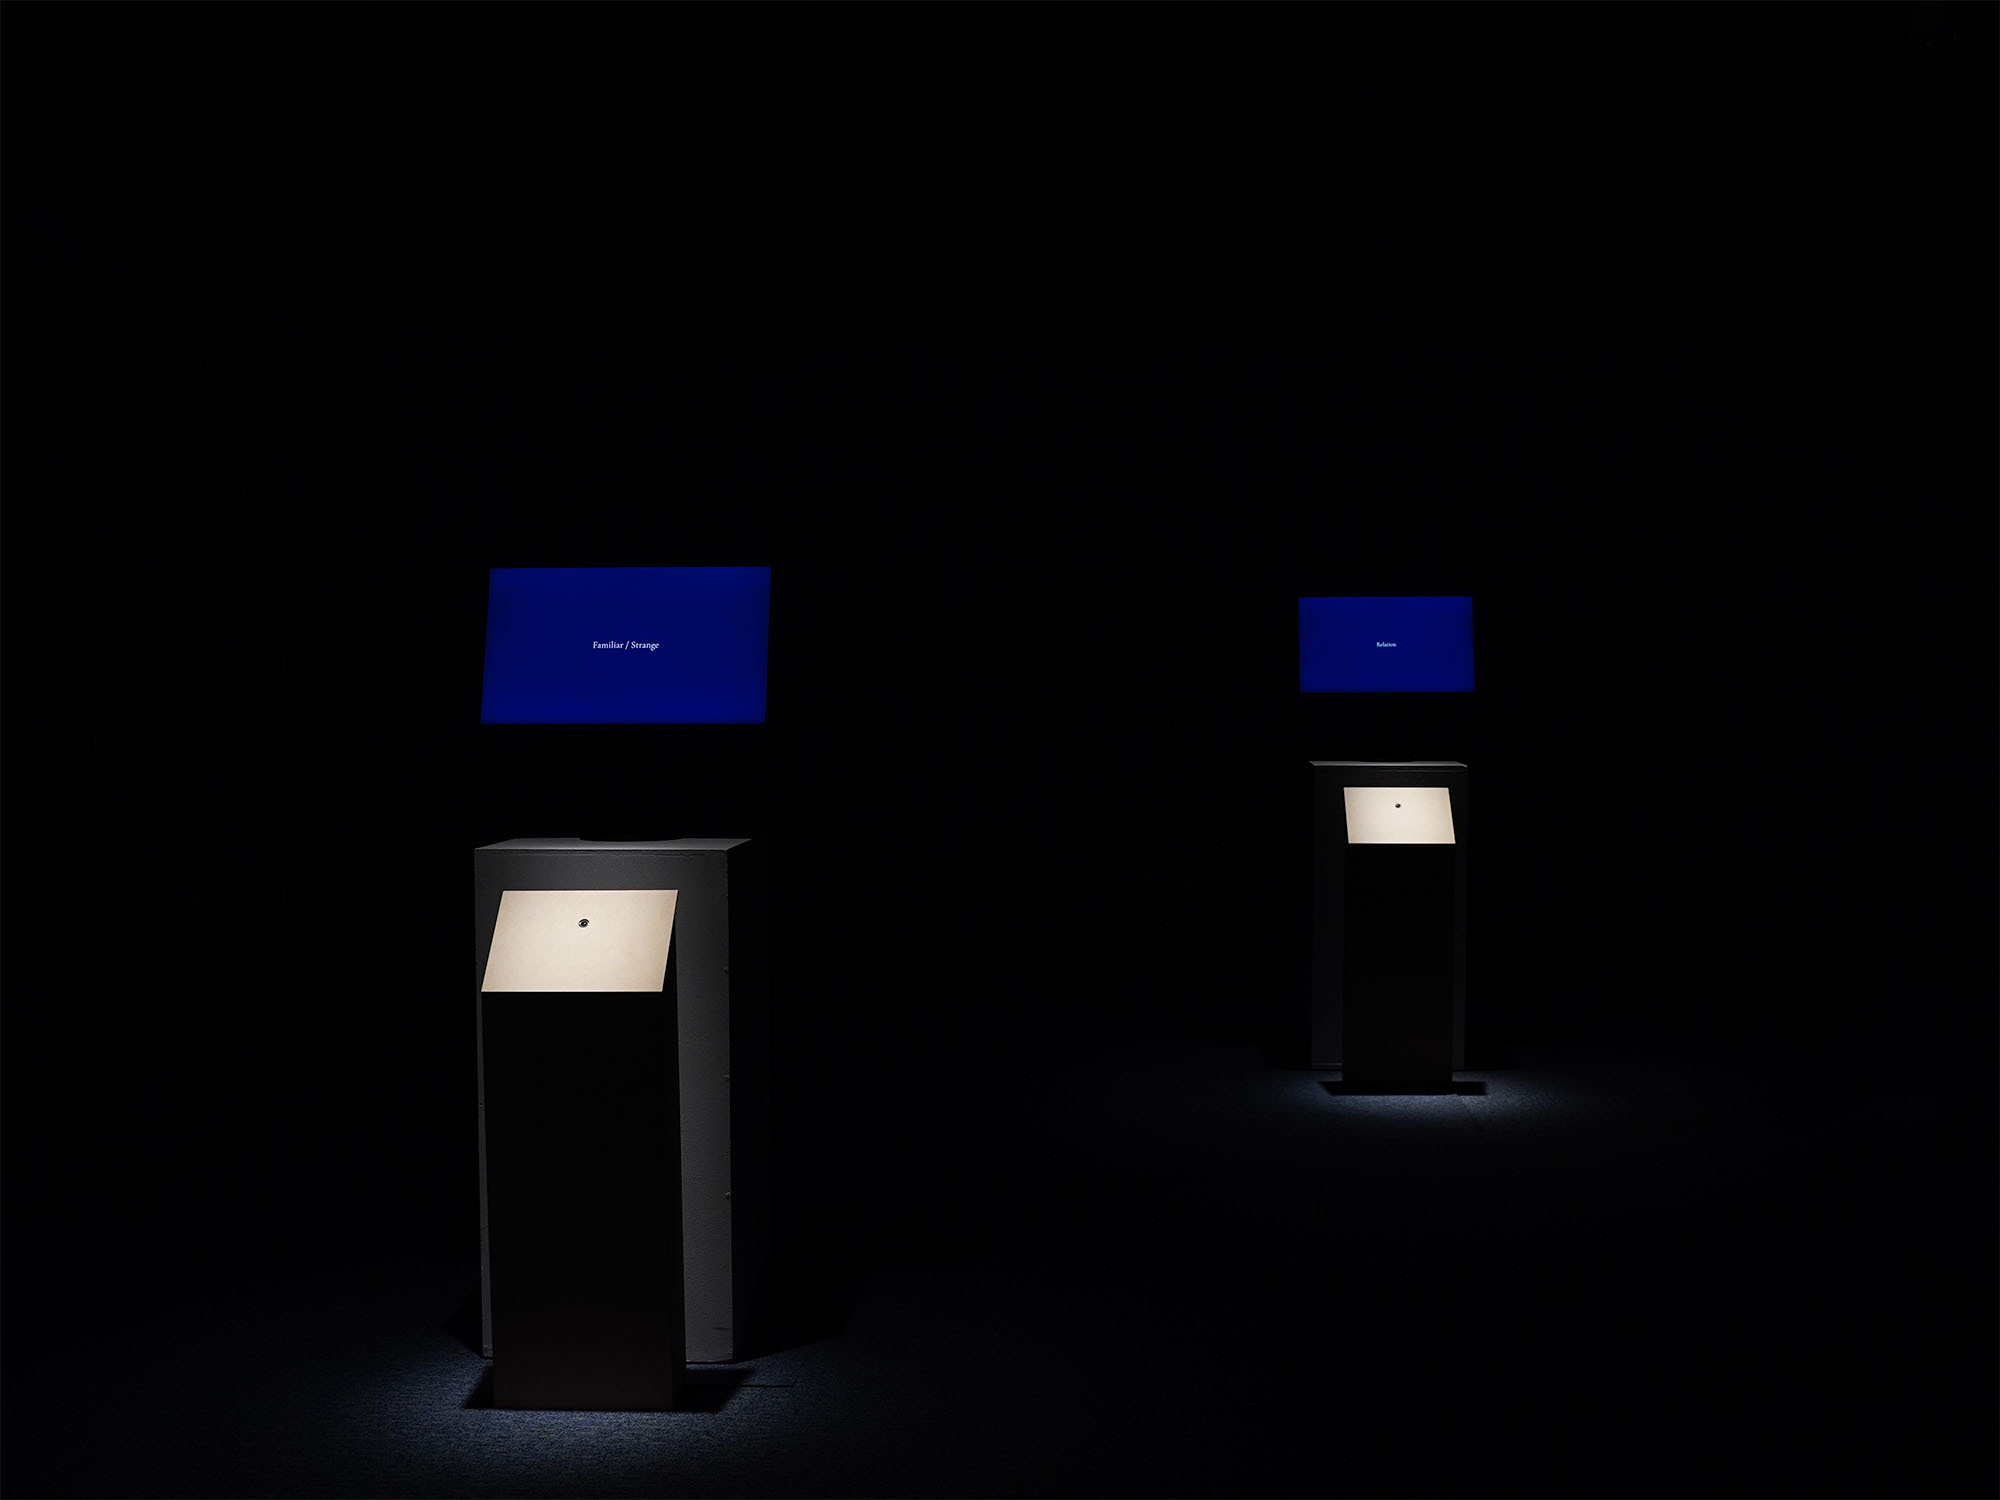
\includegraphics[width=12cm]{img/lighting.jpg}
  \caption{作品展示の際のライティング}
  \label{fig:lighting}
\end{figure}

\section{円滑な作品体験のための補助的な処理}
本作品を構成するにあたり、円滑に体験するための補完処理を実装している。具体的には、ガウシアンフィルターによる平滑化処理、トラッキングが途切れた際の例外処理の2つである。

\subsection{ガウシアンフィルターによる平滑化処理}
推定精度の問題から、モデルより推定される姿勢情報をそのまま出力すると、手指を動かしていなくても小刻みに振動したり、一時的なフレームレートの低下に起因してスムーズに動作していないように感じることがある。そこで、体験者にフィードバックする際に使用する姿勢情報は、前後2フレーム分のフレーム情報にガウシアンフィルターを適用した平滑化処理を実装している。ただし、トラッキングが開始した直後は5フレーム分のフレーム情報を使用することができないため、この場合は取得できる限りのフレーム情報を用いて同じ処理を行なっている。
% そのため以下では、各フレーム情報に対する重みづけと、それを用いて体験者に提示される姿勢情報を求める上での一般式を示す。
% モデルより推定された最新の姿勢情報を\(P_{n}\)、出力されている姿勢情報を\(S\)とすると、
%   % 平滑化フレーム S の定義
%   \begin{equation}
%     S = \sum_{i=-2}^{2} w_i' \cdot P_{n+i}
%     \end{equation}

% ここで、\(w_i'\)は正規化されたガウシアンフィルタの重みを表す。正規化前の重み\(w_i\)は、
% \begin{equation}
%   w_i = \frac{1}{\sqrt{2\pi}\sigma} e^{-\frac{i^2}{2\sigma^2}}
%   \end{equation}

% 正規化された重み\(w_i'\)は、
%   % 重みの正規化
%   \begin{equation}
%   w_i' = \frac{w_i}{\sum_{j=-2}^{2} w_j}
%   \end{equation}
% と表現される。
この処理のため、最良時で60fps程度で取得される姿勢情報は、慢性的に0.3sほどの遅延を伴って体験者にフィードバックされることになる。

\subsection{トラッキングが途切れた際の例外処理}
体験時、環境光や、手指を動かす範囲や速度の関係から、トラッキングが途切れることがある。素早い動きをしている最中に1フレームでも途切れると円滑に体験することができないため、この時は例外的に、トラッキングが途切れる直前のフレーム情報で失われたフレーム情報を埋め合わせる処理を実装した。また、トラッキングが途切れていることに起因する不快感は、本作品の体験外の問題なので、手指の動きがトラッキングできていない状態を視覚的にフィードバックするため、トラッキング不能時に塗りつぶしを透過する視覚効果を実装した(\ref{fig:track_true}, \ref{fig:track_false})。

\begin{figure}[htbp]
  \begin{minipage}[b]{0.5\linewidth}
    \centering
    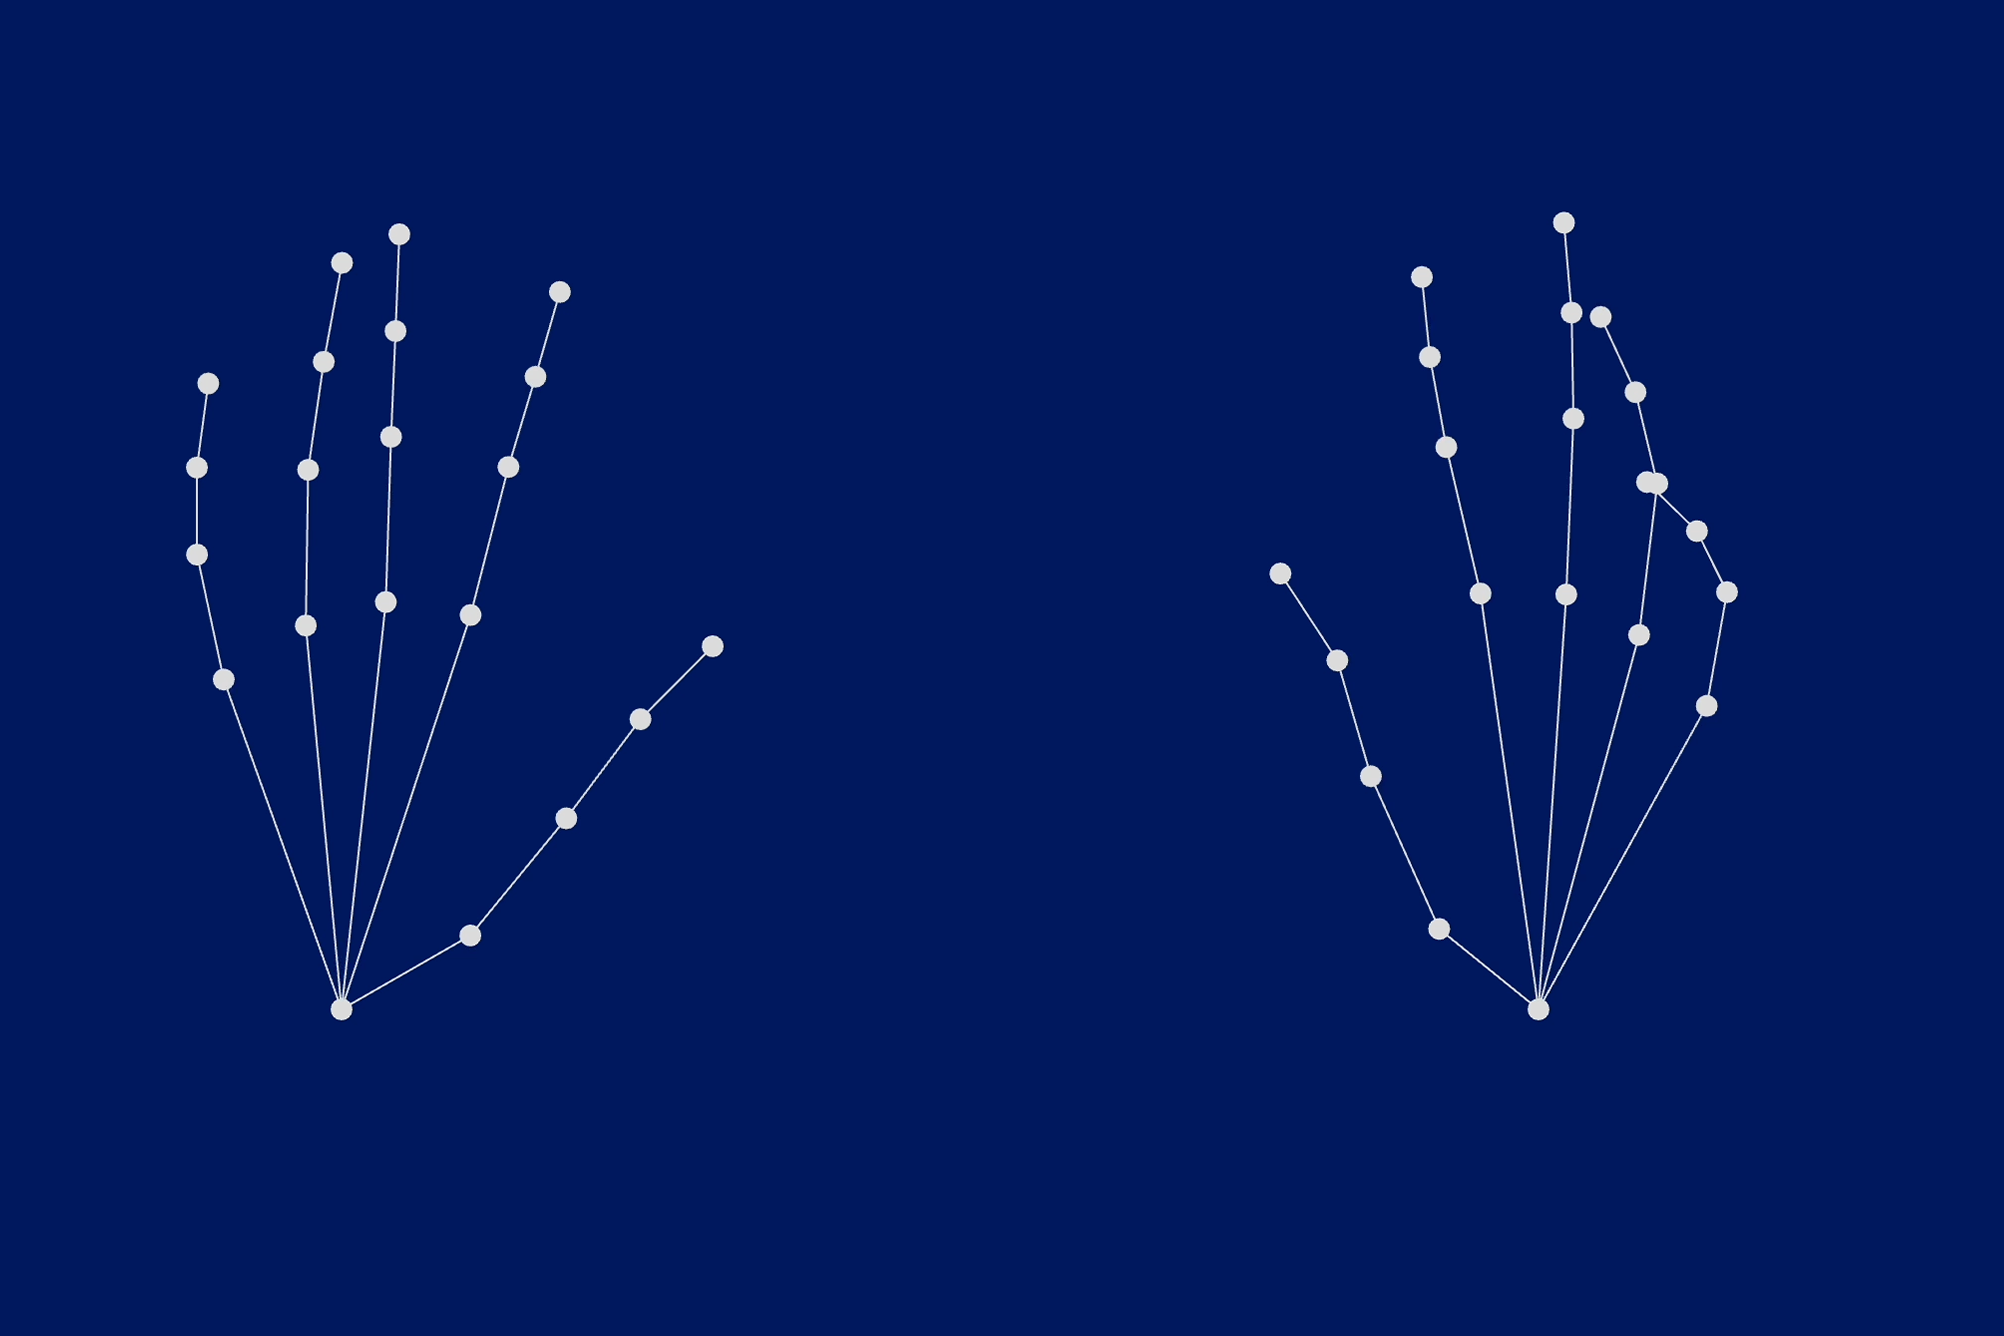
\includegraphics[keepaspectratio, width=7cm]{img/track_true.png}
    \caption{トラッキングが正常にできているとき}
    \label{fig:track_true}
  \end{minipage}
  \begin{minipage}[b]{0.5\linewidth}
    \centering
    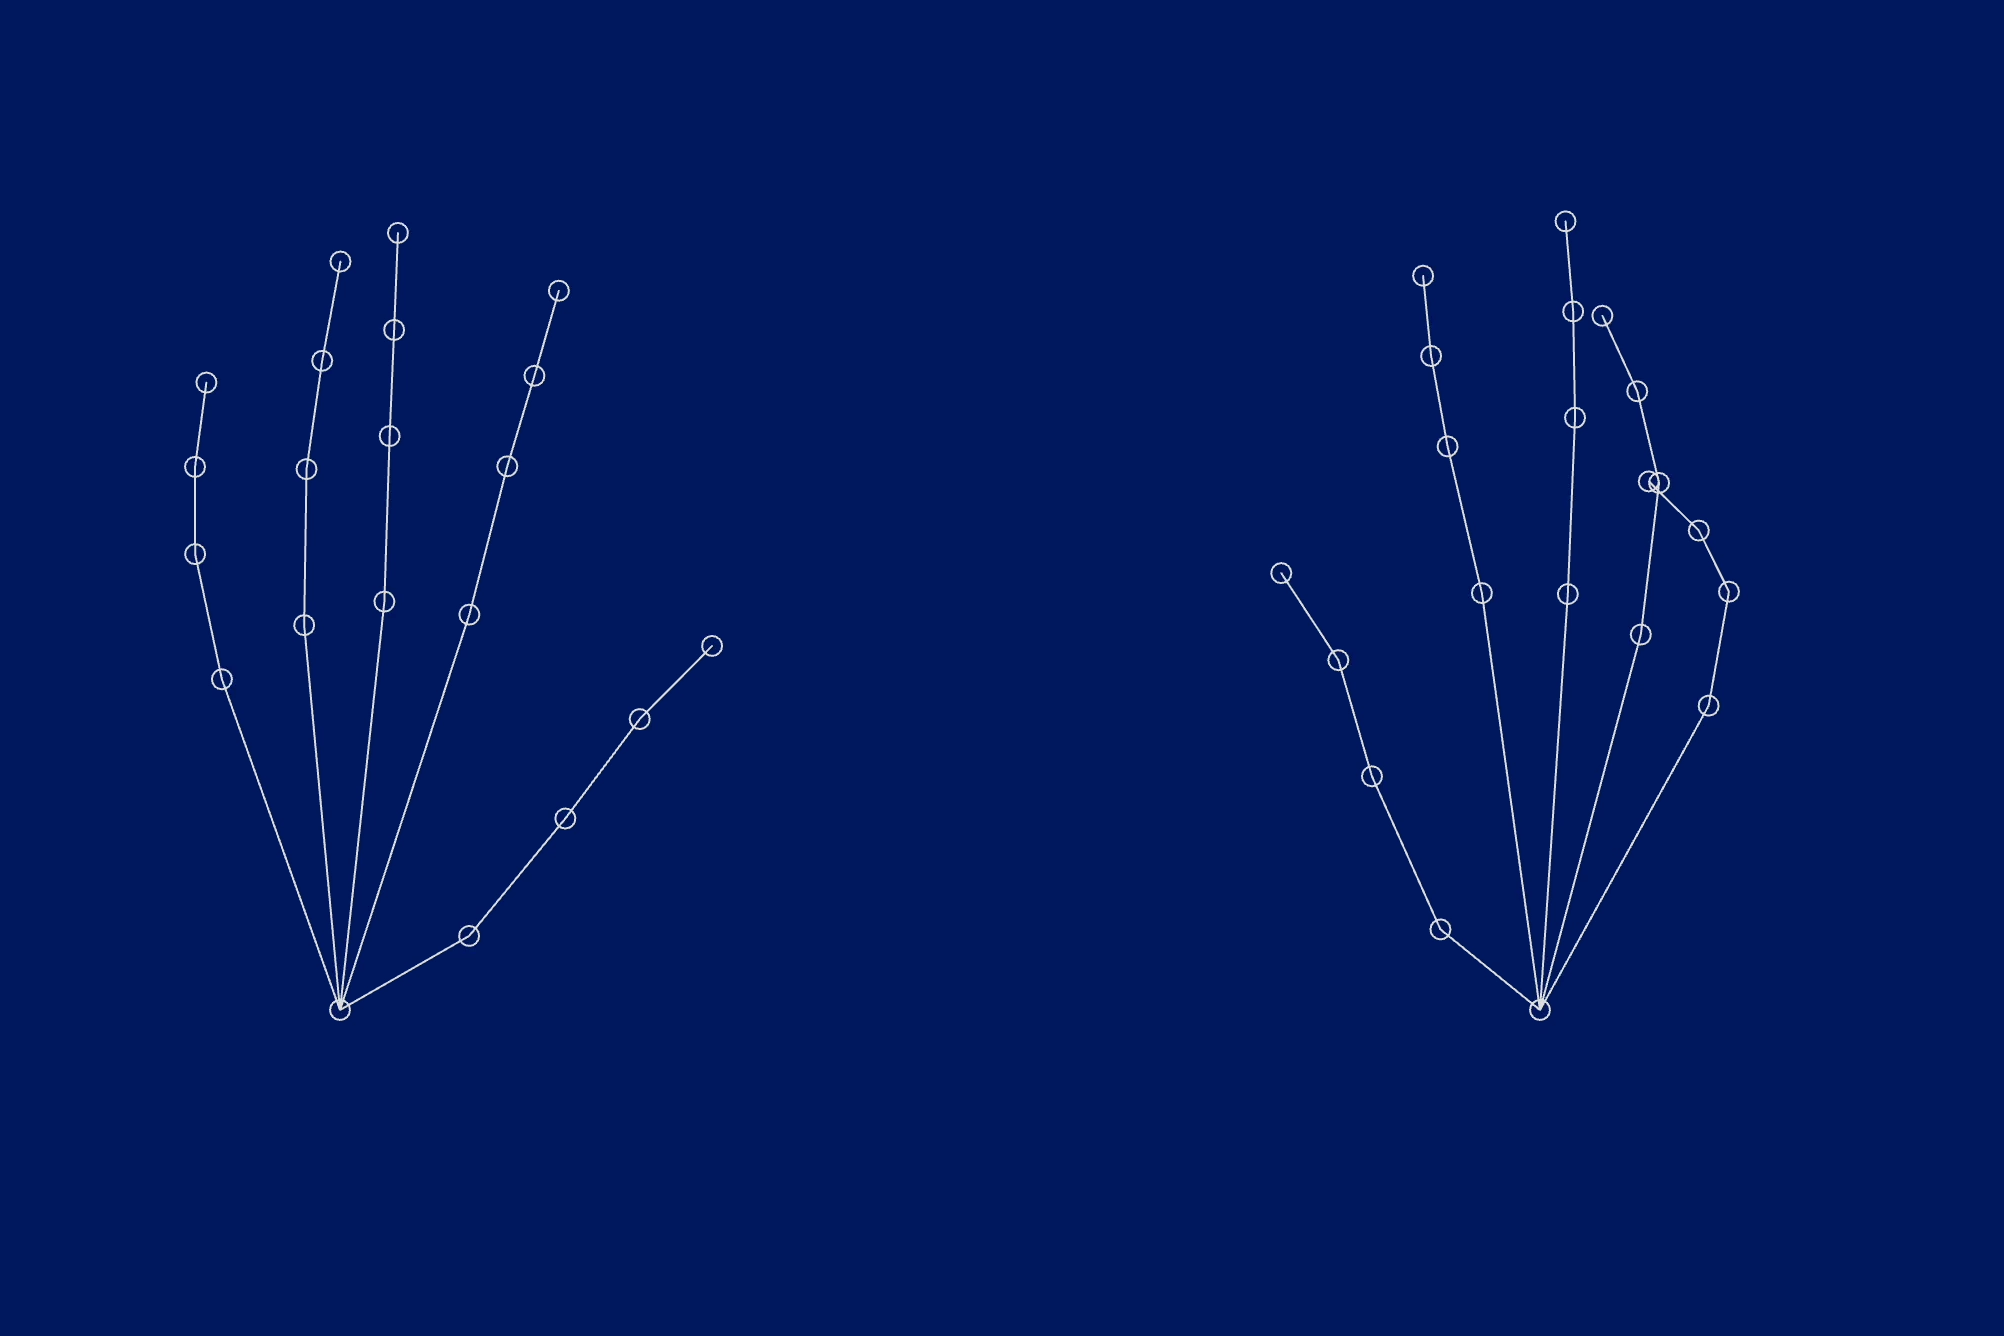
\includegraphics[keepaspectratio, width=7cm]{img/track_false.png}
    \caption{トラッキングに失敗しているとき}
    \label{fig:track_false}
  \end{minipage}
\end{figure}